% !TEX encoding = UTF-8 Unicode
% !TEX program = xelatex
% !BIB program = biber
% !TEX TS-program = xelatex
% !BIB TS-program = biber
%%
%%  本模板方式编译: XeLaTeX + biber
%%
%%  注意: 在改变编译方式前应先删除 *.toc 和 *.aux 文件
%%
\documentclass[12pt,openright]{book}

% 引入NKThesis包
\usepackage[emptydoublepage]{NKThesis}   % 中文
%\usepackage[emptydoublepage,English]{NKThesis} % 英文

% 其它包按需添加
\usepackage{amsmath}
\usepackage{cases}
\usepackage{multirow}
\usepackage{array}
% \usepackage{tocbibind}
\usepackage{ulem}
% \usepackage{subfigure}

\usepackage{xeCJKfntef} %CJKunderline
\xeCJKsetup{underline= {format = \color{black}, thickness=0.4pt}} %CJKunderline setting

% 参考文献
\addbibresource{nkthesis.bib}
% 图片文件夹
\graphicspath{{image/}}

\includeonly{
	./tex/abstract,
	./tex/introduction,
	./tex/method,
	./tex/experiments,
	./tex/summary,
	./tex/references,
	./tex/acknowledgements
}
\begin{document}
%  设置基本信息
%  注意:  逗号`,'是项目分隔符. 如果某一项的值出现逗号, 应放在花括号内, 如 {,}
%
\NKTsetup{
	% 封面设置
	论文题目(中文) = 面向协同线性流形学习的实验设计与分析,
	论文题目(英文) = Experimental Design and Analysis for Collaborative Linear Manifold Learning,
	学号           = 1511413,
	姓名       = 陈齐翔,
	年级          = 2015级,
	学院          = 软件学院,
	系别          = 软件工程,
	专业          = 软件工程,
	完成日期      = 2019年5月26日,
	指导教师       = 谢茂强\ 副教授,
}


% !TeX root = ../main.tex
% -*- coding: utf-8 -*-


\begin{zhaiyao}

近年来,网络数据量已呈爆炸式增长,人们每天都产生着海量的数据。如何有效利用这些数据,
从中挖掘出有价值的信息帮助人们认识世界成为了一个重要课题,链接预测问题也由此产生。


链接预测可以挖掘出网络中丢失的链接或进行网络动态分析,是机器学习领域中的一个重要课题。
随着相关研究的深入,人们对算法的需求愈加复杂,例如需要算法有对层次结构数据或带有辅助信息数据的处理能力,或是能使用序列化输入的方式训练模型。
本文的研究目的之一就是如何有效利用辅助信息以提高模型的预测精度。
由于现实数据的维度往往很高,直接使用时模型的训练成本较高,
考虑到数据通常为嵌入在高维空间的低维流形结构,本文首先提出了一个基于线性流形学习的算法来解决高维数据的问题。
在此基础上,本文又利用辅助信息,使用同样地方式构建了一个双流形结构,利用两个流形结构的一致性提出了一个双边协同学习算法。
算法通过协同学习的方式令两个流型相互补全,成功利用辅助信息解决了由数据稀疏带来的流型结构不完整的问题。


此外,虽然近年来涌现了众多优秀的算法,但一个很常见的问题就是与算法相关的实验较匮乏,
因此,本文的另一个研究目的就是从不同角度设计实验来检验算法性能和分析影响因素。
为了检验算法性能,本文对算法做了交叉验证、鲁棒性检验、后续检验,并最终发现所提算法与其它算法相比,性能有显著提升;
为了分析影响算法性能的因素,文中又从数据的结构上出发,设计了多个实验并做了解释分析;
为了验证算法在实际应用中的有效性,文中最后将该算法应用到了对药物间关联的预测中并得到了令人满意的结果。
\end{zhaiyao}


\vspace{20pt}

\begin{guanjianci}
链接预测;流形学习;协同学习;实验设计
\end{guanjianci}



\begin{abstract}


In recent years, the amount of data in network has exploded and people can generate massive amounts of data every day. 
How to utilize those data, digging out some useful information buried underground to give us a hint of real world, 
has become an important subject and thus generating a problem called link prediction.


Link prediction can be used to extract missing information, identify spurious interactions, evaluate network evolving mechanisms, and so on. 
So that it can be used in recommendation systems, Pathogenic gene mining and drug interaction mining. 
In this article, a linear manifold learning algorithm has been devised to uncover novel interactions on a global scale 
since data are usually embedded in low-dimensional manifolds. Then a collaborative learning method has been introduced 
with the help of auxiliary information to solve the problem of data sparsity.


To evaluate the overall performance of our method and find out some relationships between network topology structure 
and predicting results, several experiments have been carried out. In the cross validation experiments, 
our method achieved better results than eight other state-of-the-art methods in most cases and has better robustness. 
Finally, we loaded some real DDI data to test our method and found that it predicted the left-out interactions reasonably well.

\end{abstract}


\vspace{20pt}


\begin{keywords}
link prediction; manifold learning; collaborative learning; experimental design and analysis
\end{keywords} 

\tableofcontents

% !TeX root = ../main.tex
% -*- coding: utf-8 -*-
% !TeX root = ../main.tex
% -*- coding: utf-8 -*-

\chapter{绪论}
\label{chpt:introduction}

链接预测的相关研究不仅有着重要的理论意义,能大力推动其它相关领域研究的进展,而且具有广泛的应用场景。
近年来,随着网络科学的快速发展,其理论上的成果为链接预测搭建了一个研究的平台,
使得链接预测的研究与网络的结构与演化紧密联系起来,
使得预测结果能从理论的角度上给出更合理的解释。
除此之外,链接预测的研究也可以从理论上帮助人们认识复杂网络的演化机制。
针对同一类网络,很多模型都提供了可能的网络演化机制\cite{吕琳媛2010复杂网络链路预测},
但描述网络拓扑结构的统计特征非常多,不仅很难比较哪个特征描述的更准确,
而且仅凭一两个特征往往很难从整体上刻画网络。
而链接预测机制有望为其提供一个简单统一且较为公平的比较平台,
从而大大推动复杂网络演化模型的理论研究。

\section{网络链接预测的背景}

在自然界和人类社会中广泛存在着各种各样的复杂系统,
这些复杂系统都可以用复杂网络的形式很好的表示出来。
网络中的点代表一个独立个体,
网络中的链接可代表个体间的关系或相互作用。
例如,互联网可以看作是由路由器或者接入Internet的计算机通过光纤等通信介质相互链接所形成的网络;
信息网络可以看作是信息的发送者和接收者之间通过信息传播路径所链接的关系网络;
生物体中的神经系统可以看作是大量的神经细胞通过神经纤维相互链接所形成的网络;
此外,还有社会关系网络、电力网络、科学家合作网络、蛋白质相互作用网络、交通网络等等。
因此,复杂网络的研究不仅对现实生活有非常重要的意义,对人类了解自然界和社会的发展也有着长远的科学指导意义,
而链接预测便是复杂网络研究中很重要的工作。\cite{刘宏鲲2011利用链路预测推断网络演化机制}

链接预测是通过利用网络的拓扑结构、节点属性等信息来预测网络内两个不相连的点是否会建立链接。
通常来说要预测的链接分为两种:一是已存在但未被发现的链接,二是未来可能产生建立的新链接\cite{李淑玲2012基于相似性的链接预测方法研究}\cite{wang2017novel}。


\section{链接预测的实际应用}
\subsection{链接预测在社交网络中的应用}
\label{intro:sec:social}
一个社交网络就是一个由社会中的个体以及这些个体间的关系构成的庞大社会结构。
可以把社交网络看作一个图,图中的节点表示社会中的个体,链接就表示个体间的关系或产生的交互\cite{李淑玲2012基于相似性的链接预测方法研究}。
目前,各类社交软件诸如微信、微博或Facebook等已逐渐成为人们日常生活中的一部分,
人们可借此平台方便的与他人分享信息,而由此也产生了一个庞大且复杂的社交网络,
且网络中海量的数据又有着质量高、数据量大、是现实社会关系的真实映射等很有价值的特点,
因此这些数据也吸引了来自不同领域的众多学者的目光\cite{wang2015link}。

\begin{figure}[h]
  \subfigure[Stanford 社交网络]{
    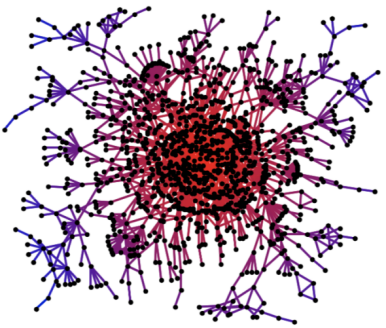
\includegraphics[]{stanford_social_net.png}
  }
  \subfigure[MIT 社交网络]{
  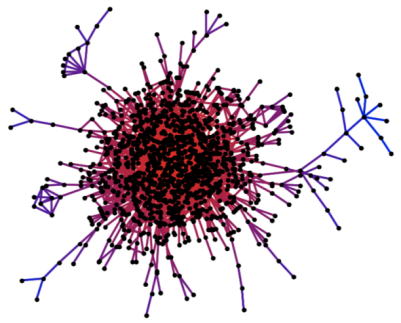
\includegraphics[]{MIT_social_net.png}
  }
  \caption{社交网络示意}
  \label{intro:fig:social_net}
\end{figure}
Lada A. Adamic 和Eytan Adar在2003年通过分析大学中学生的个人主页构建出了一个小型社交关系网络\cite{adamic2003friends}。
他们观察到,学生经常会在自己的个人主页中提及自己的朋友,
而这主要是通过使用超链接指向对方的个人主页或在朋友列表中列出对方的邮件地址;
此外,个人主页中的某些文本也可以用来揭示社交关系,例如有两个人在自己的主页中都提到了“机器学习”这门课程,
那么这两人便有可能因为在同一间教室上课而成为朋友。
作者分别使用MIT和斯坦福大学中的个人主页成功构建出了两个社交网络,
其中每个学生作为一个节点,节点间的链接是通过分析了上述几个信息源后标注出的。
图\ref{intro:fig:social_net} 展示了两所大学内的社交网络。


\begin{center}
\tablecaption{对Chao.C.H的预测结果}
\begin{tabular}{c|c|c}\hline
\multicolumn{3}{c}{CAnakken: Clifford Hsiang Chao}\\ \hline
是否为朋友 & 相似度 & 姓名\\ \hline
否 & 8.25 & Eric Winston Liao\\
是 & 3.96 & John Andrew Vestal\\
否 & 3.27 & Desiree Dawn Ong \\
是 & 2.82 & Stanley Hsinheng Lin\\
否 & 2.66 & Daniel Sunil Chai \\
否 & 2.55 & Wei Nan Hsu \\
是 & 2.42 & David J.Lee \\
否 & 2.41 & Hands Christian Andersen \\
否 & 2.41 & Byung Joo Lee\\ \hline
\label{intro:table:chao}
\end{tabular}
\end{center}


为了预测某两人是否为朋友,文中对每两个人之间的相似度做了排序然后直观的给出结论:
两个人间相似度越高就越可能是朋友。在定义了合适的相似度计算方式后便得到了所有人互相成为朋友的概率。
表\ref{intro:table:chao} 以名为Clifford Hsiang Chao的学生为例给出了他与前九名相似度最高的学生的真实关系,
从中可以看出,算法在保证了一定准确率的同时也提供了潜在的可能成为朋友的人。

\subsection{链接预测在医学中的应用}
链接预测在医学界的一个典型应用就是对药物-药物相互作用(Drug-Drug Interaction, DDI)的预测。
DDI是导致药物潜在危害反应的一个重要原因,尤其是在当病人同时摄入多种药物的时候\cite{fokoue2016predicting}。
例如最近的研究显示,老年人是最常见的同时摄入多种药物的群体,并且大约在每25人中就会有一个人受到过因DDI产生的危害\cite{huang2013systematic}\cite{juurlink2003drug}。
再比如用于临床治疗患有情绪障碍(如重度抑郁症)的患者时常使用的三环类抗抑郁药物也被认为会经常引起药物间反应,
一是由于这类患者往往患有其它伴随病症从而需要服用多种其它药物,二是情绪障碍类疾病的治疗周期很长,
即需要长时间服用药物。如今的许多处方药,如“拜新同”(一种降压药),都会在其药品说明书中列出与其它类药物共同使用时可能发生的反应。

因此,发现和预测DDI不仅可以预防临床用药时发生的不良反应,还可以帮助开出含有共同药物的处方以提供更好的治疗效果\cite{zhang2018prioritizing}。
虽然前人已经做了很多努力去寻找可能的DDI并将已知信息存入到了数据库中,如:KEGG、DrugBank以及STITCH。
但最近的研究显示,没有一种数据源能涵盖所有的DDI,而且大部分的数据源要么不完整要么就是保守地列出了许多“无关痛痒”的DDI\cite{fokoue2016predicting}。
而近些年出现的一个新研究方向是基于药物本身的机制、结构信息或与蛋白质的相互作用来预测新型DDI。
预测方法类似于在研究社交网络时使用的计算相似性的方法。\cite{vilar2012drug}通过计算药物间分子结构的相似性来预测DDI,其基于的假设就是,
如果药物A与药物B具有相似的分子结构,则那些会与A发生有害反应的药物也很有可能与B也产生相似反应。
举例来说,据Medical Literature研究显示,辛伐他汀是一种通过抑制HMG-CoA还原酶来降低胆固醇水平的药物,
可以与三唑类抗真菌药物氟康唑相互作用,导致肌病或横纹肌溶解症的风险增加;则根据文中的假设,
那些类似于辛伐他汀的药物也可以与氟康唑相互作用并产生如上所述的类似的相互作用。
图\ref{intro:fig:process}以此为例展示了主要的计算过程。

\begin{figure} 
  \centering
  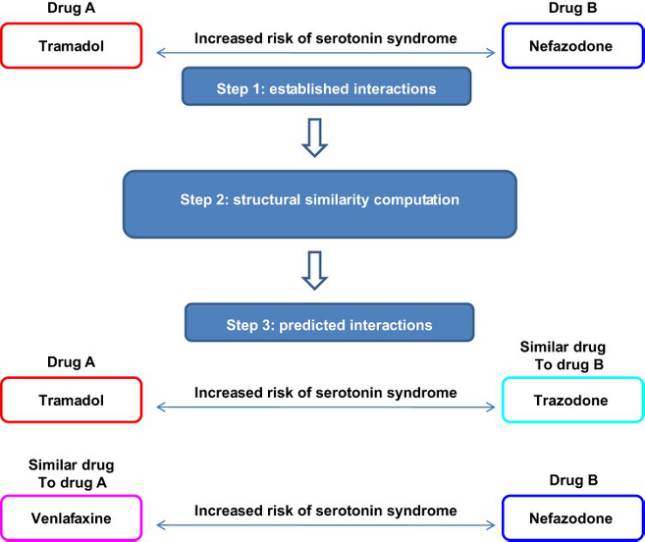
\includegraphics[width=8cm, height=8cm]{example_predict_process.png}
  \caption{以分子结构作为相似度的计算过程\cite{vilar2012drug}}
  \label{intro:fig:process}
\end{figure} 

图\ref{intro:fig:result}举例列出了算法在2009年售出最多的50种药中预测出的相互作用,它们尚未被DrugBank验证。

\begin{figure} 
  \centering
  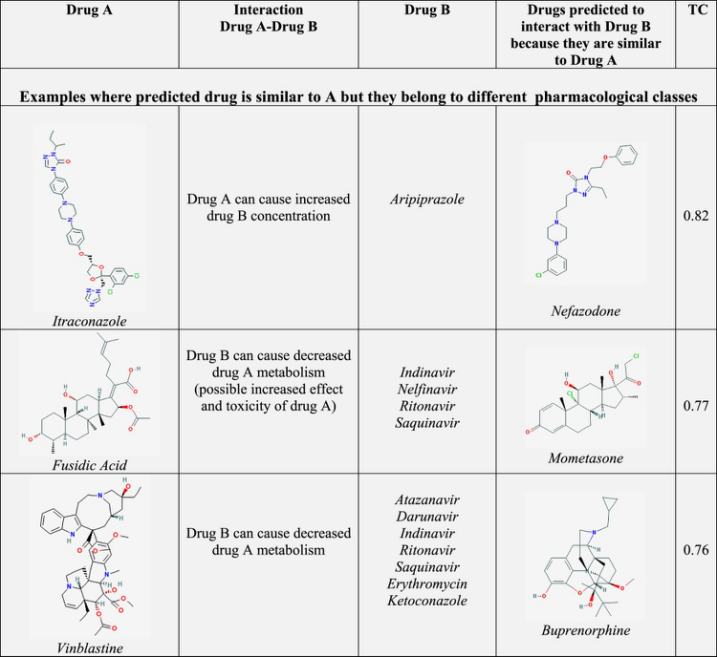
\includegraphics[width=8cm,height=9cm]{example_predict_result.png}
  \caption{对实际药物的预测结果举例\cite{vilar2012drug}}
  \label{intro:fig:result}
\end{figure} 

\subsection{链接预测在其他领域中的应用}
除上述两个典型场景外,链接预测算法也在其他领域有着广泛的应用:
在电子商务中链接预测可以用来构建推荐系统;
在图书馆科学中,可以利用链接预测来删除重复数据;
在信息检索领域中,为提高检索效率,可以利用链接预测技术改进搜索引擎和信息检索的超文本分析\cite{李淑玲2012基于相似性的链接预测方法研究};
除此之外链接预测还可以用来判断学术论文的类型、判断手机用户是否产生了切换运营商的念头\cite{李淑玲2012基于相似性的链接预测方法研究}或者重新规划航班线路。


\section{国内外研究现状}
\label{intro:sec:study}
目前的链接预测算法主要分为三类:基于相似度的、基于路径的和基于矩阵分解的方法\cite{lu2009similarity}。本节将简单介绍各类别方法中的一些经典算法。

\subsection{基于相似度的方法}
在所有基于相似度的算法中,
Common Neighbors(CN)算法和\ref{intro:sec:social} 节提到的Adamic-Adar(AA)算法可谓最具代表性的两个算法。
前者将节点间相似度定义为两节点间共同邻居(即相同邻接点)的个数;
后者在这之上对邻接点的度数做了惩罚以减弱“富人俱乐部”效应,两个算法都成功做出了链接预测。
在这之后,许多基于这两个方法的新算法如雨后春笋般被提出来,它们要么是在原算法的基础上做了改动,要么是使用了CN或AA的结果作为相似度的依据之一。


陈槿慧等人在2015年使用信息论的方法提出了一个基于共同邻居集合的算法,叫做NSI。
该算法在面对具有多重结构特征的数据时很有效。NSI从信息论的角度衡量了网络中拓扑结构的特点,不同的拓扑结构含有不同的隐含信息并进而影响到对链接的预测\cite{chen2014robust}。


Scellato等人在药物-药物关联预测领域提出了一个网络连通性指标(network-connectivity score)来衡量药物和对应靶蛋白间关系的强弱。
略具体来说,算法使用了三种数据:药物-药物关联数据、药物-蛋白关联数据以及蛋白-蛋白关联数据,
然后算法利用药物-蛋白关联数据将药物映射到了蛋白网络中,通过对蛋白网络中药物相关节点集的系统连通性进行评分,计算目标网络中节点对的相似度\cite{scellato2011exploiting}。


\subsection{基于路径的方法}
基于路径的链接预测算法更多关注网络的拓扑结构信息,Katz提出了一个经典算法来计算节点对之间所有的潜在路径,
其损失函数中对路径长度做了惩罚,即越长的联通路径损失越大\cite{elhamifar2013sparse}。


张平等人提出了一个称为LP的标签传播算法\cite{zhang2015label},该算法将相似性的使用分为一阶和二阶来链接具有相同标签的节点。
除了用于目标网络的标签传播算法之外,损失函数由从不同辅助信息导出的各个相似性矩阵线性组合。


徐中启等人用信息论的方法量化了节点路径特点对链接预测的影响并以此提出了一个用于预测用户社交关系的算法。
算法通过引入辅助数据“用户对不同地理位置的到访记录”,计算出了一个路径熵(Path Entropy)指标,依此做链接预测\cite{xu2016link}。

\subsection{基于矩阵分解的方法}
Menon等人提出使用监督矩阵分解方法解决图中的链接预测问题,
他们综合考虑了(从目标网络中分解得到的)隐含特征、节点本身的特征以及链接的特征,算法使用了随机梯度下降的方法优化\cite{singh2008relational}。


Singh等人为进一步提升预测准确率而综合考虑了数据中的多种关系,将其统一后给出了新的矩阵分解公式,
当对由不同关系形成的多个矩阵进行分解时,不同元素的系数会根据情况来“共享”。


曹珠等人将矩阵补全和子图嵌入思想结合起来进行表征学习。其中,子图嵌入用于捕获细粒度的节点特征,凸矩阵补全用于去除噪声和迭代地提高泛化能力\cite{cao2018link}。


Guimerà等人提出了一种称为MCLP的替代迭代算法来解决矩阵补全问题,目标网络被视为缺失的数据集,并通过矩阵补全从拓扑结构信息中恢复潜在的链接\cite{guimera2009missing}。

\section{论文组织结构}
本论文一共分为四章,其中二、三章为论文主体部分,各章内容分别为:


第一章为绪论,主要介绍了链接预测问题的背景、举例介绍了相关算法在实际问题中的应用然后简要分析了国内外在该领域的研究进展。


第二章介绍算法,提出了协同线性流形学习算法并给出各部分的推导过程。


第三章为实验部分,首先介绍了实验所用的数据来源,简单分析了数据集的结构特点,介绍了实验常用的评价指标,然后详细介绍了引入的一系列实验并分别做了实验分析。


总结了算法的性能并展望了今后工作中可能的着手点。
% !TeX root = ../main.tex
% -*- coding: utf-8 -*-

\chapter{协同线性流形学习算法介绍}
\label{chpt:method}
协同线性流形学习(Collaborative Linear Manifold Learning,CLML)是一个基于流形学习做链接预测的算法。
该算法首先假设了数据空间是一个低维嵌入,利用辅助矩阵和目标矩阵分别学习到了两个流形,通过“两个流形具有一致性”这个假设定义出了带低秩约束的损失函数;
最后,算法使用随机梯度下降对模型进行优化。图\ref{method:fig:CLML}以药物-药物关联预测为例展示了算法的主要流程,本章将分小节介绍该算法的各个部分。

\begin{figure} 
  \centering
  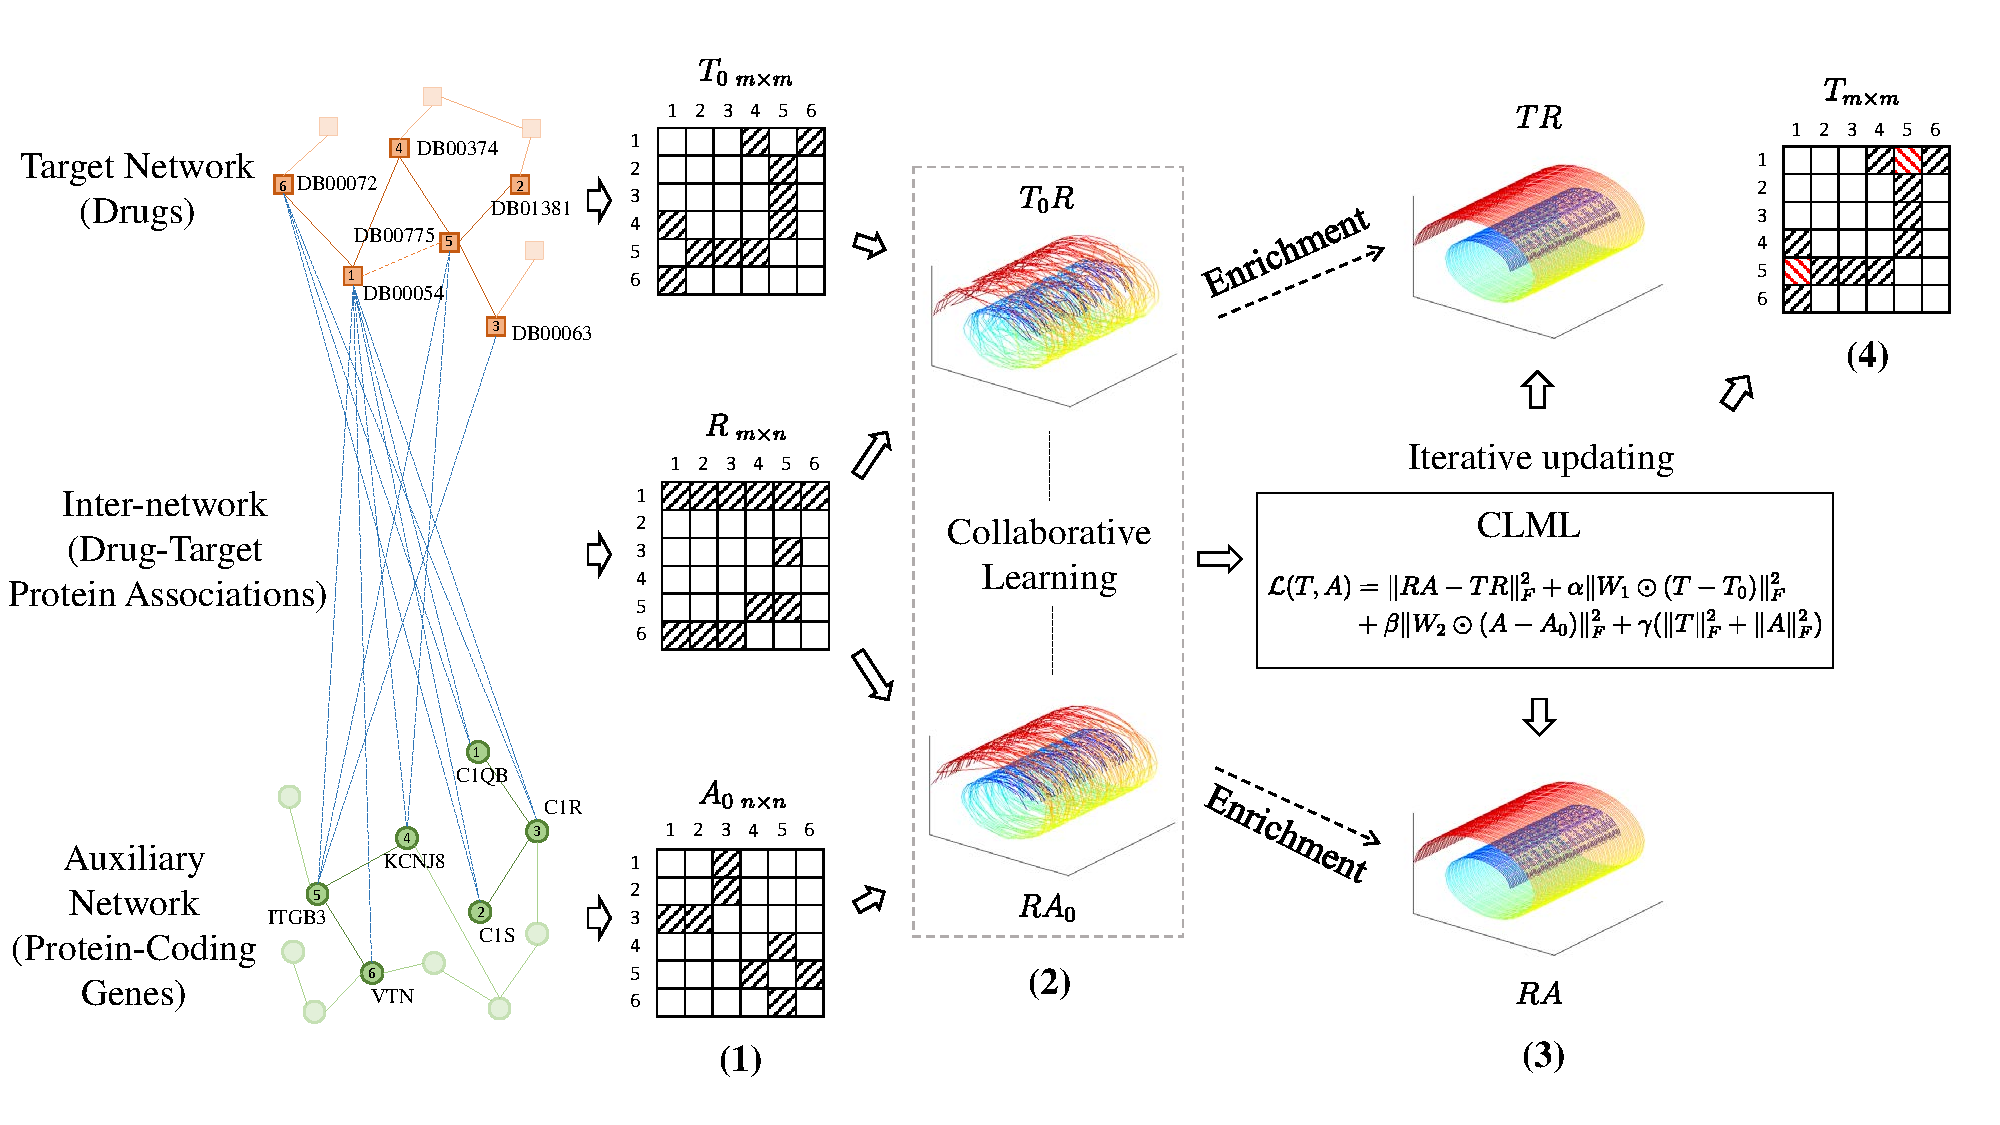
\includegraphics[width=15cm, height=9cm]{CLML.pdf}
  \caption{CLML算法主要流程}
  \label{method:fig:CLML}
\end{figure} 


\section{符号表示}
\label{method:sec:notations}

为了简化算法推导过程中对所用符号的解释并保持上下文符号一致性,本节总结了将要用到的所有重要符号并做了解释,各符号意义参见表\ref{method:table:notations}。

\begin{center}
\tablecaption{各符号释义}
\begin{tabular}{l|l} \hline
    符号 & 意义 \\ \hline
    $m$         & 目标矩阵的规模 \\
    $n$         & 辅助矩阵的规模 \\
    $D_{m*m}$   & 目标矩阵 \\
    $R_{m*n}$   & 网络间关联矩阵 \\
    $T_{n*n}$   & 辅助矩阵 \\
    $I_n$       & $n*n$的单位矩阵 \\
    $\Arrowvert{X}\Arrowvert_{F}$ & X的Frobenius范数 \\
    $\Arrowvert{X}\Arrowvert_{*}=\sum_{i}\sigma_i$ & $X$的核范数 \\
    $\sigma_i$  & 矩阵第i大的奇异值 \\
    $X\odot{Y}$ & $X$与$Y$的哈达玛积 \\
    $\langle{X},\ Y\rangle$ & X与Y的内积 \\ \hline
\end{tabular}
\label{method:table:notations}
\end{center}

目标矩阵就是我们要对其预测的矩阵,辅助矩阵就是算法中引入的辅助信息对应的矩阵,网络间关联矩阵就是这两各矩阵间的关系。
如在DDI预测中,药物-药物关联矩阵就是目标矩阵,蛋白-蛋白关联矩阵就是辅助矩阵,药物-靶蛋白关联矩阵就是网络间关联矩阵。


\section{线性流形学习}
\subsection{先验约束}
\label{method:subsec:prior}
流形学习(manifold learning)是一类借鉴了拓扑流形概念的降维方法,它把数据看作是一个嵌入在高维空间中的低维结构。
因此,虽然数据维度可能很高或在高维空间分布很复杂,但在局部却仍具有欧式空间的性质,可利用欧式距离重新进行距离测算,
在局部建立降维映射关系来将数据映射到低维空间中。


局部线性嵌入(Locally Linear Embedding,LLE)是流形学习的一个著名算法。
LLE假设,在高维空间中的任意一个点,在局部范围内(它的k近邻点)近似位于一个超平面上,
所以该样本点可以通过其k近邻点的线性组合重构出来,即空间中的一点满足式(\ref{method:formula:self_repre})。


\begin{equation}
    \hat{X_i}=\sum_{j\in\phi(i)}\omega_{ij}X_j \label{method:formula:self_repre}
\end{equation}

其中,$\phi(i)$表示点i的k近邻点集合,$\omega_{ij}$为线性重构时每个点的权重系数,为$\omega_{ij}$找到合适的值后便可令每个点都由其近邻点线性表出。


LLE算法的不足之处在于,当数据过于稀疏时容易产生“断路”,即某些点无法找到k个足够近的近邻点。
而稀疏子空间聚类(Sparsity Subspace Clustering,SSC)算法认为,
在一个子空间内的每个点都可以由其余所有点线性表出\cite{elhamifar2013sparse}。
因此为了应对数据稀疏的问题,CLML在LLE的基础上,将重构过程扩展到了全局范围内,
即每个点均使用其余所有点来线性表出而不再仅使用其k近邻点,即使其余点并未与该点直接相连,如图\ref{method:fig:global_manifold}所示。

\begin{figure}
    \centering
    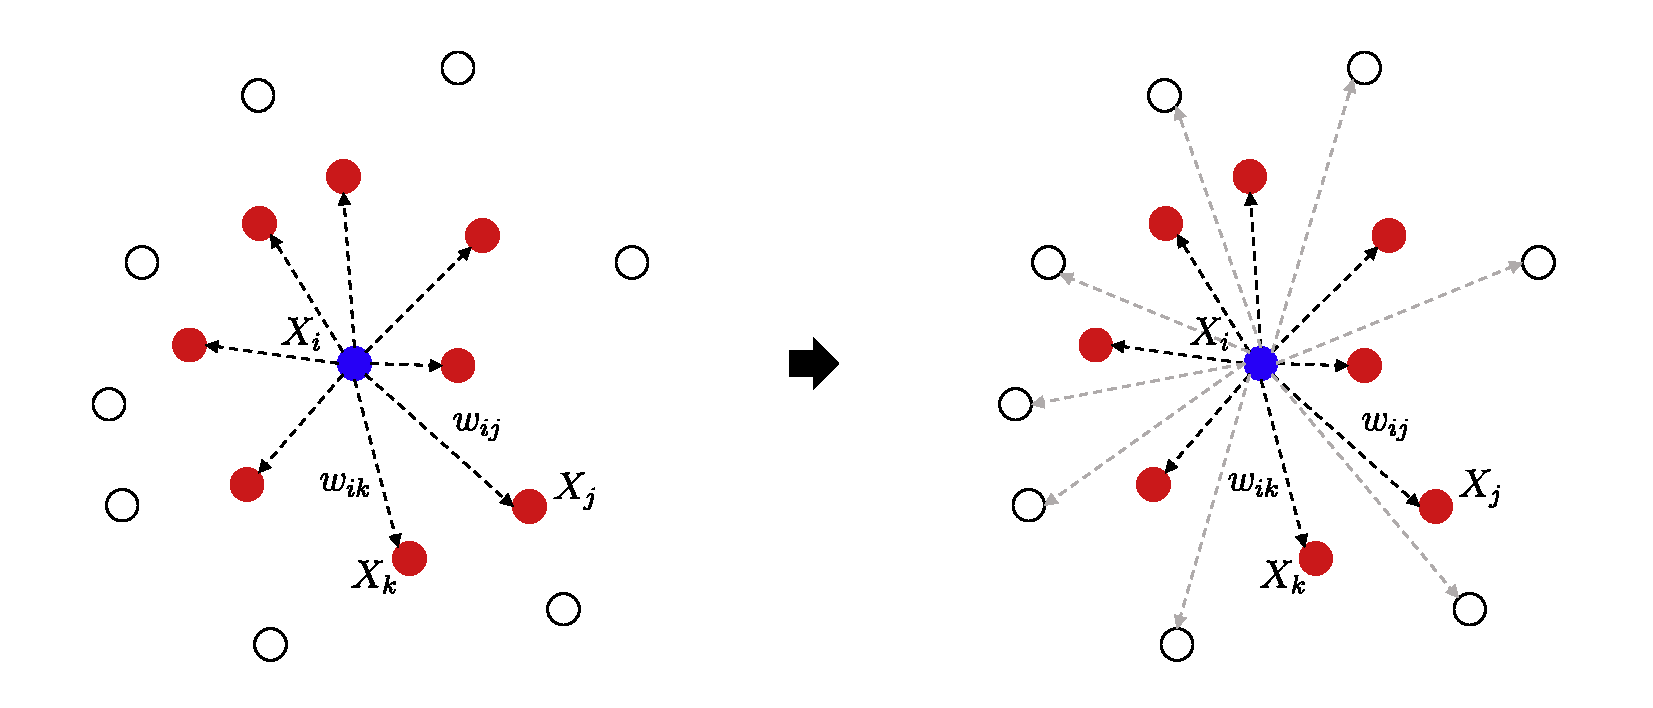
\includegraphics[width=15cm, height=6cm]{global_manifold.pdf}
    \caption{将构建流形使用的点扩张至全局范围内}
    \label{method:fig:global_manifold}
\end{figure}

因此我们得到了式(\ref{method:formula:constraint})中的对先验数据的约束,其中$W_{ij}$便是为了控制与点相连和不相连的点在重构时的权重。
$W_{ij}$的取值如式(\ref{method:formula:weight})所示,里面的$\mu$是一个介于[0, 1]内的可调节的参数,为了让直接相连的点在重构时权重更大,通常令$\mu\geq0.5$;
是一个足够大的数来保证矩阵对角线元素接近0,这保证了每个点只能由其余点来表示(而不是用自己表示)。

\begin{equation}
    f(D)=\sum^m_{i=1}\sum^m_{j=1}W_{ij}(D_{ij}-D_{0ij}) \label{method:formula:constraint}
\end{equation}


\begin{equation}
    W_{ij}=\begin{cases}
        \mu,& if\ \ D_{0ij} = 1 \\
        1 - \mu,& if\ \ D_{0ij} = 0 \\
        \rho,& if\ \ i = j
        \end{cases}
        \label{method:formula:weight}
\end{equation}


我们大费周章地将$D_0$矩阵中每个点都用其余点表示的目的,就是为了让之后预测出的新矩阵$D$与原矩阵$D_0$尽可能接近,从而进行链接预测的。

\subsection{重构线性流形}

在上一小节中我们得到了用$D$矩阵近似表示$D_0$所用的约束,接下来我们需要提出具体的损失函数,依靠损失函数我们才能最终学习到具体的$D$矩阵。


我们观察到,矩阵$D$、$R$的结构类似,也就是说使用$D$线性重构$R$矩阵后得到的结果仍为$m*n$的矩阵,且仍代表网络间的相互关系。
于是,我们利用这一特点对$R$和$R*D$的近似做了约束。为了防止过拟合,我们还加入了对矩阵$D$的正则化项,最终得到式(\ref{method:formula:simple_ver})。


\begin{align}
L(D)&=\sum_{i=1}^m\Arrowvert{R_i-\sum_{j\neq{i}} R_jD_{ij} }\Arrowvert^2 + 
\alpha\sum_{i=1}^m\sum_{j=1}^mW_{ij}(D_{ij}-D_{0ij})+\gamma\Arrowvert{D}\Arrowvert_F^2\nonumber \\
    &= \Arrowvert{R-RD}\Arrowvert_F^2+\alpha\Arrowvert{W}\odot(D-D_0)\Arrowvert_F^2+\gamma\Arrowvert{D}\Arrowvert_F^2
    \label{method:formula:simple_ver}
\end{align}

式中,$\alpha$和$\beta$为超参,分别控制先验数据的约束项和正则项对损失函数的影响。最终学习到的$D$矩阵中的每个元素将是一个在[0, 1]范围内的连续数值,
做预测时可再令$P=(\arrowvert{T^*}\arrowvert+\arrowvert{T^{*^T}}\arrowvert)/2)$即可得到一个对称矩阵$P$,
其中$P_{ij}$的值代表节点$i$和节点$j$产生链接的概率,$P_{ij}$越大则两点间越可能产生链接。


\subsection{低秩约束}

如果一个矩阵的秩远小于它的维数,则可称为低秩矩阵。低秩也代表着矩阵行、列间的相关性很强,可以互相线性表出,
该特性可很好的运用在特征分析或矩阵补全(如图像修复、链接预测等)上,而在\ref{method:subsec:prior}节中提到,需要让矩阵$D$中的每个点均由其余点线性表出,
因此可以通过引入低秩约束来更好地满足这一需求。为保持矩阵低秩,可对矩阵使用$L0$范数约束,但$L0$范数的优化是个NP难问题,
故我们使用核范数来近似,也即令式(\ref{method:formula:simple_ver})中的F范数替换为$\Arrowvert{D}\Arrowvert_*^2$。


\section{协同学习}
\label{method:sec:collaborative}
在上一节中利用$R$和$R*D$的相似性已经可以对目标矩阵进行链接预测了。但实验发现,$R$矩阵往往较为稀疏,
仅利用$R$和$R*D$之间的相似性得到的预测结果并不好,且观察后发现$R$和$R*D$之间仅有50\%左右的相似性。


但注意到,辅助矩阵$T$和$R$同样具有相似的结构,使用$T*R$组合得到的新的矩阵同先前使用$D$矩阵时一样,都应和$R$矩阵近似,因此可以很快推导出式(\ref{method:formula:dual_ver})。

\begin{align}
L(T)&=\sum_{i=1}^m\Arrowvert{R_i-\sum_{j\neq{i}} T_{ij}R_j }\Arrowvert^2 
+\alpha\sum_{i=1}^m\sum_{j=1}^mW_{ij}(T_{ij}-T_{0ij})+\gamma\Arrowvert{T}\Arrowvert_*^2 \nonumber \\
    &=\Arrowvert{R-TR}\Arrowvert_F^2+\alpha\Arrowvert{W}\odot(T-T_0)\Arrowvert_F^2+\gamma\Arrowvert{T}\Arrowvert_*^2
    \label{method:formula:dual_ver}
\end{align}


值得注意的是,在式(\ref{method:formula:simple_ver})和式(\ref{method:formula:dual_ver})中使用的是同一个R矩阵。我们令$R_d=R*D$和$R_t = T*R$,则$R_d$和$R_t$都应与矩阵$R$近似,区别仅在于二者使用的是不同的先验数据。
既然$R_d$和$R_t$都与同一个$R$近似,那么理论上$R_d$和$R_t$也应具有一致性,即$R_d \approx R_t$。基于此,我们提出了如式(2.6)所示的协同学习算法的损失函数,
式中$W_1$、$W_2$的取值和作用与式(\ref{method:formula:simple_ver}), 式(\ref{method:formula:dual_ver})相同,$\alpha$、$\beta$仍为超参。
\begin{align}
L(D,\ T)=&\Arrowvert{RD-TR}\Arrowvert_F^2+\alpha\Arrowvert{W_1}\odot(T-T_0)\Arrowvert_F^2 \nonumber\\
        &+\beta\Arrowvert{W_2}\odot(D-D_0)\Arrowvert_F^2+ \gamma(\Arrowvert{T}\Arrowvert_*^2+\Arrowvert{D}\Arrowvert_*^2)
\end{align}
通过协同学习的方式我们可以克服$R$矩阵数据稀疏导致重构后两矩阵差异较大(仅50\%)的问题。
通过实验发现,使用协同学习后$R_d$和$R_y$能达到接近98\%的相似度,这足以说明引入协同学习的必要性和算法的实际效果。

\section{本章小节}
本章首先提出了一个基于线性流形学习的算法,但实验后的效果并未达到预期。之后我们又考虑了辅助信息,在原来算法的基础上引入了协同学习来克服数据稀疏的影响。
% !TeX root = ../main.tex
% -*- coding: utf-8 -*-

\chapter{实验设计与分析}
在本章中我们将对CLML算法展开一系列实验,希望通过对比,得到CLML算法的准确率、鲁棒性等指标,以及它在实际应用中的表现,并试图从数据集的特点上探究影响算法性能的因素。 


\section{实验数据与参数设置}
\subsection{评价指标}
在分类问题中,我们经常会计算出样本在每个类别下的概率,这样做可通过设置阈值来满足对模型的不同需求。
例如,(在二分类问题中)当阈值设为0.5时,所有输出概率在[0, 0.49]范围内的样本将被标记为负类(Negative),
在[0.5, 1.0]的样本便被标记为正类(Positive)。根据样本的真实类别与算法预测类别的组合可将样本划分为四类,
分别为:真正例(True Positive,TP)、假正例(False Positive,FP)、真反例(True Negative,TN)、假反例(False Negative,FN)。
据此,我们可得到表\ref{experiments:table:mix_matrix}中的“混淆矩阵”,它表明样本是否被错误分类,是评估分类算法的基础。
\zihaowu
\begin{center}
    \tablecaption{混淆矩阵}
    \begin{tabular}{ccc} \hline
        \multirow{2}{*}{真实情况} & \multicolumn{2}{c}{预测结果} \\ \cline{2-3}
                                & 正例  & 反例  \\ \hline
        正例                     & 真正例(TN)   & 假反例(FN) \\ 
        反例                     & 假正例(FP)   & 真反例(TN) \\ \hline
    \end{tabular}
    \label{experiments:table:mix_matrix}
\end{center}
\zihaoxiaosi
\begin{enumerate}
    \item ROC:ROC曲线全名为Receiver Operating Characteristic curve,即“受试者工作曲线”,是衡量二分类算法的一个常用指标。
    曲线画出了当阈值在[0.0, 1.0]范围内变化时,模型真正例率(True Positive Rate,TPR)和假正例率(False Negative Rate,FNR)的变化情况。
    TPR和FNR分别定义为:
    \[ TPR = \frac{True Positives}{True Positives + False Negatives} \]
    \[ FPR = \frac{False Positives}{False Positives + True Negatives} \]
    ROC在二分类算法中经常被使用的原因为:首先,可在ROC曲线图中直观地对比不同的算法;其次,ROC曲线下的面积(AUC)可作为模型性能的总结[26]。
    \item AUC:AUC\cite{hanley1982meaning}(Area Under Curve of ROC)是评估模型预测结果质量时经常使用的一个指标。AUC的取值范围为[0, 1],值越大代表分类器越好。
    次。一个较简单的计算公式为:
    \[AUC=\frac{1}{mn}\sum^m_{i=1}\sum^n_{j=1}1_{p_i>p_j}\]
    其中,$m$表示所有的真正例样本数量$n$表示所有的真负例样本数量,$1_{p_i>p_j}$则表示赋予真正例样本的概率大于真负例样本概率的个数。
    \item AUC20:由于我们的算法更加侧重于预测出的高概率链接,因此我们限制预测出的FP数量要小于等于20,并将该结果也作为一个评价指标。
    \item AUPR:AUPR\cite{davis2006relationship} 全称为Area Under curve of Precision-Recall,其中查准率P(precision)和查全率R(recall)分别定义为:
    \[P=\frac{TP}{TP+FP}\] \[R=\frac{TP}{TP+FN}\]
    显然查准率和查全率是一对相互矛盾的度量(P高时R往往偏低,反之亦然)。
    类似于画ROC曲线的方式,PR曲线描述了当阈值变化时查准率和查全率的关系,曲线下方的面积(AUPR)提供了对正确预测出正类和负类比例的量化性评估\cite{van2011gaussian}。
    由于在链接预测问题中,负类样本数量往往远多于正类样本,而AUPR又更多地惩罚FP类的样本,因此AUPR是一个比AUC更有价值的测量指标\cite{van2011gaussian}.
\end{enumerate}


\subsection{数据集介绍和交叉验证实验}
\label{experiments:sec:db_cv}
实验时我们从四个完全不同的领域挑选出了四个数据集,分别为:
\begin{enumerate}
    \item Douban Movie数据集:Douban Movie是国内一个知名的影评网站\footnote{https://movie.douban.com/},用户可在网站上对任意电影从1至5打分;
    此外,用户还可添加好友,进行一定程度的社交。又因为不同电影可以根据类别、演员、语种甚至上映日期分类,
    故我们可选定一些特征将电影分类,规定某一类中的电影是彼此相似的。通过在该网站爬取上述信息,
    我们便可构建出用户-用户关联矩阵$D$、用户-电影关联矩阵$R$以及电影-电影关联矩阵$T$。
    \item Yelp数据集:Yelp是国外一个很常用的商户点评网站\footnote{http://www.yelp.com/dataset challenge/},用户可在其上对到访过的商户打分、评论以供后人参考。
    使用类似处理Douban数据集的方法,我们同样可以获得$D$、$R$、$T$矩阵。
    \item NIPS合作数据集:NIPS合作数据集包含了在特定科研领域中发表的论文与其作者,以及最具特点的:不同作者间相互合作的关系。
    例如,若作者A和作者B共同参与发表了一篇论文,则可认为A和B进行了一次合作。该数据集也因此受到了来自不同领域学者的广泛关注。
    \item DDI数据集:如第一章所述,DDI表示不同药物在临床共同使用时是否会发生相互作用。
    与之类似,DPI(Drug-Protein Interaction)网络代表药物对与靶蛋白之间的关系(许多药物都是通过影响特定蛋白质的合成来治疗疾病的)、
    PPI(Protein-Protein Interaction)代表蛋白质与蛋白质间的作用(许多疾病、基因表型往往是多种蛋白共同作用的结果)。
    Drugbank是一个权威的生物医学信息网站,其每一两个月就会统计各文献、临床报告中发现的新的DDI、DPI和PPI,
    整理后发布到其官网\footnote{https://www.drugbank.ca/releases}上供学者研究。
\end{enumerate}


需要指出,原始数据包含许多其它信息且格式不统一,我们使用的均是由\cite{zhang2018prioritizing}提供的清洗后的数据。


表\ref{experiments:table:simple_stats}初步统计了从四个数据集中构建的$D$、$R$、$T$矩阵的特点。
从表格中可以粗略看出Douban数据集的样本数最多(A、B数量均高于其他数据集),
但A-A关联矩阵却较为稀疏;相反,DDI数据集包含的样本数量很少(采样成本远高于其他三个),
但A-A矩阵有近四分之一的非零元素;Yelp数据集中不仅样本数量大,且矩阵也含有相对较多的非零元素。


为进一步帮助理解数据集的特点,我们又分析了每个数据集中节点度数的分布(图\ref{experiments:fig:node_distribution}),
并统计了每个数据集的聚类系数、平均度数、网络直径等分析复杂网络常用的统计指标,见表\ref{experiments:table:topo_stats}。

\zihaowu
\begin{center}
    \tablecaption{对四个数据集的初步统计数据}
    \begin{tabular}{@{\extracolsep{\fill}}p{2.5cm}<{\centering}p{2.5cm}<{\centering}p{2.5cm}<{\centering}p{2.5cm}<{\centering}p{2.5cm}<{\centering}}\hline
        数据集        & Douban & Yelp & NIPS & DDI \\ \hline
        关系(A-B)   & 用户-电影 & 用户-商家 & 作者-出版物 & 药物-靶蛋白 \\
        A的数量       & 13367   & 16239  & 2865  &  758  \\
        B的数量       & 12677   & 14284  & 2484  &  473  \\
        A-A的数量     & 4085    & 158590 & 63178 & 11852 \\
        A-B的数量     & 168278  & 198397 & 5879  & 2296  \\ \hline
    \end{tabular}
    \label{experiments:table:simple_stats}
\end{center}

\begin{figure}[]
    \centering
    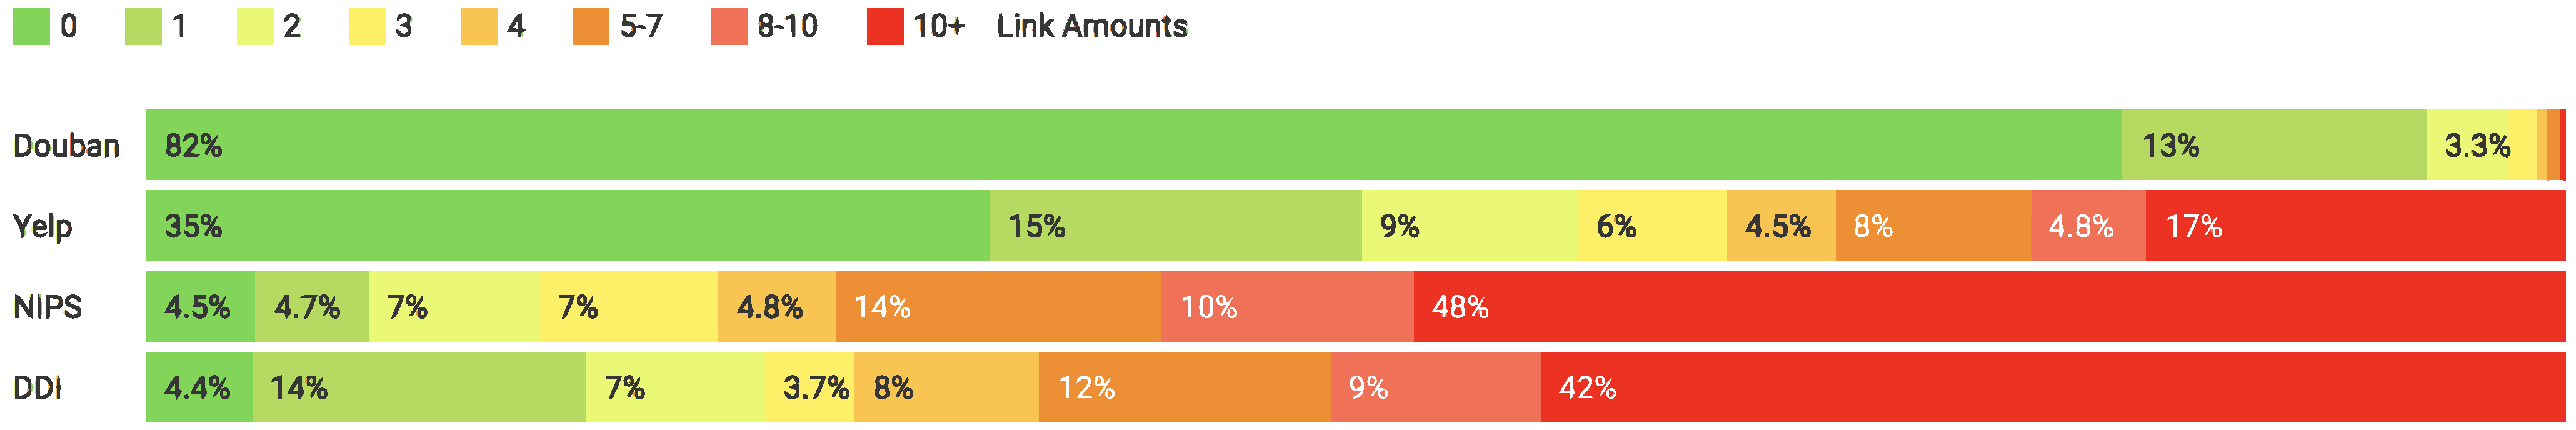
\includegraphics[width=0.98\linewidth, height=3cm]{node_distribution.pdf}
    \caption{各数据集节点度数分布}
    \label{experiments:fig:node_distribution}
\end{figure}


\begin{center}
    \tablecaption{各数据集拓扑结构的详细信息}
        \begin{tabular}{p{2.5cm}<{\centering}p{2.5cm}<{\centering}p{2.5cm}<{\centering}p{2.5cm}<{\centering}p{2.5cm}<{\centering}}\hline
            数据集          & Douban & Yelp & NIPS & DDI \\ \hline
            聚类系数        & 0.017 & 0.226 & 0.609 & 0.164 \\
            网络密度       & 0.001   & 0.001  & 0.009  &  0.023  \\
            网络直径     & 29   & 11  & 11  &  7  \\
            平均近邻数     & 1.948  & 14.990 & 23.048  & 16.348  \\ \hline
        \end{tabular}
        \label{experiments:table:topo_stats}
\end{center}
\zihaoxiaosi
实验时,我们随机选取80\%的数据作为训练集,记录并删掉剩余的20\%数据作为测试集,然后用在训练集上的预测结果与测试集做对比。
模型训练时使用5*10折交叉验证,即我们将训练集随机划分为10份,每轮依次使用其中的1份作为验证集,剩余的9份作为训练集,
重复5次取平均数作为本次模型的结果,代码3.1为交叉验证的关键代码:



\begin{lstlisting}[caption={交叉验证的关键代码},language=Matlab]
    function [ result ] = CrossValidationOf-
    DualManifoldWithLowRank(R, D, W1, T, W2, alpha, beta, gamma,
     maxIterator, fold,density)
    % m 是矩阵 R 的行数
    [m, ~] = size(R); 
    % base 是每折的样例数
    base = floor(m / fold); 
    % result 保存计算出的每折的平均 AUC 和 AUPR
    result = zeros(fold, 2); 
    
    % iterate process 具体的迭代过程
    for i = 1:fold % 分别对每一折进行计算
        lastNum = base * i; % 每一折的末尾行号
        beginNum = lastNum - base + 1; % 每一折的开始行号
        
        trainData = D; % 同时抹去 D 中这一折的行和列,
        trainData(beginNum:lastNum, :) = 0; % 作为训练集
        trainData(:, beginNum:lastNum) = 0;       
        T = eraseData(T,density);
        % 学习得到预测的 D = |D| + |D'|;
        predictData = abs(DualManifoldWith-
        LowRank(R, trainData, W1, T, W2, alpha, beta,
         gamma, maxIterator));
        predictData = predictData + predictData';
       .......
        % 一折结束
    end
    result = mean(result, 1); % 对最后的结果求平均
    end
\end{lstlisting}

\subsection{对比算法}
在\ref{intro:sec:study}中我们提到,链接预测算法大致分为三类,因此我们从这三类中分别挑选出了一些比较有代表性的算法。
我们在基于相似度的算法中选取了CN、AA、NSI算法;
在基于路径的算法中选取了LP、MCLP;
在矩阵分解算法中选取了MF、MRMF算法;
除此之外,我们称未引入协同学习时的算法为LML,将其也作为一个对比算法来一并研究协同学习在算法中的作用。

\section{实验设计与分析}
\subsection{算法性能结果}
我们分别使用四个数据集对CLML算法和其它对比算法进行测试,在选取了最佳参数后,
我们得到了表\ref{experiments:table:auc20}~\ref{experiments:table:aupr}中的数据,
表中加粗的结果代表每个数据集下取得的最大值。从中我们可以看出,基于线性流形学习的方法,无论是LML还是CLML都较大部分算法而言有明显提升;
而使用了两个线性流形进行协同学习的CLML与LML相比更是在各项指标中均有显著提升,在AUPR上甚至提升了近50\%。
注意到,MRMF算法在Yelp数据集中的AUC20要优于LML和CLML,但该算法的AUC和AUPR却均低于我们的算法。
因此我们可以初步得出结论:CLML算法的性能优于其它对比算法。


此外,从各算法的AUC值可以看出,基于特征提取(feature extraction)、标签传播(label propagation)的算法在链接预测问题上并不适用,
AUC值接近甚至低于0.5,因为这些算法并没有利用辅助信息也没有考虑到数据的结构特点。
与之相反,CLML不仅利用了数据集中的辅助信息,也考虑了数据的流形结构和低秩特性,这也是CLML在此类数据集上的优点。 
\zihaowu
\begin{center}
    \tablecaption{各算法的AUC20值对比}
    \begin{tabular}{ccccc} \hline
        算法 & Douban & Yelp & NIPS & DDI \\ \hline
        CN  & 0.0213 & 0.0568 & 0.0193 & 0.0161 \\
        AA  & 0.0290 & 0.0282 & 0.0173 & 0.0251 \\
        NSI & 0.1725 & 0.2088 & 0.1751 & 0.2879 \\
        LP  & 0.0569 & 0.2447 & 0.1066 & 0.3643 \\
        MCLP& 0.1528 & 0.1321 & 0.0511 & 0.0837 \\
        MF  & 0.1949 & 0.2895 & 0.1722 & 0.1760 \\
        MRMF& 0.1574 & \bfseries 0.3545 & 0.1481 & 0.3679 \\ \hline
        LML & 0.1349 & 0.0843 & 0.1990 & 0.1584 \\
        CLML& \bfseries 0.3014 & 0.2070 & \bfseries 0.2281 & \bfseries 0.5436 \\ \hline
    \end{tabular}
    \label{experiments:table:auc20}
\end{center}


\begin{center}
    \tablecaption{各算法的AUC值对比}
    \begin{tabular}{ccccc} \hline
        算法&	Douban & Yelp & NIPS & DDI \\ \hline
        CN  & 0.5186 & 0.5804 & 0.5038 & 0.5121 \\
        AA  & 0.5248 & 0.5489 & 0.5057 & 0.5388 \\
        NSI & 0.6474 & 0.6731 & 0.6097 & 0.6437 \\
        LP	& 0.5520 & 0.6969 & 0.4621 & 0.7136 \\
        MCLP& 0.6904 & 0.7269 & 0.6357 & 0.7322 \\
        MF  & 0.6710 & 0.6884 & 0.5895 & 0.6503 \\
        MRMF& 0.6658 & 0.7475 & 0.6243 & 0.8186 \\ \hline
        LML & 0.6551 & 0.6358 & 0.6210 & 0.8040 \\
        CLML& \bfseries 0.7203 & \bfseries 0.7808 & \bfseries 0.6438 & \bfseries 0.8297 \\ \hline
    \end{tabular}
    \label{experiments:table:auc}
\end{center}

\begin{center}
    \tablecaption{各算法的AUPR值对比} 
    \begin{tabular}{ccccc} \hline
        算法 &	Douban & Yelp & NIPS & DDI \\ \hline
        CN  & 0.0115 & 0.0229 & 0.0171 & 0.0292 \\
        AA  & 0.0085 & 0.0141 & 0.0170 & 0.0322 \\
        NSI & 0.0870 & 0.1273 & 0.1160 & 0.1506 \\
        LP	& 0.0285 & 0.1341 & 0.0927 & 0.3490 \\
        MCLP& 0.0519 & 0.0750 & 0.0398 & 0.0795 \\
        MF  & 0.1043 & 0.2266 & 0.1137 & 0.0814 \\
        MRMF& 0.0744 & 0.2548 & 0.1269 & 0.3679 \\ \hline
        LML & 0.1622 & 0.1370 & 0.1717 & 0.3287 \\
        CLML& \bfseries 0.2488 & \bfseries 0.2642 & \bfseries 0.1751 & \bfseries 0.3917 \\ \hline
    \end{tabular}
    \label{experiments:table:aupr}
\end{center}
\zihaoxiaosi
\subsection{后续检验}

通过观察数据初步得出了CLML优于其它算法的结论,但仅凭比较测试结果的大小还远不足以下最终定论,主要有以下几个原因:
第一,实验数据是在测试集上的结果,而我们希望比较的是模型间的泛化性能,二者有一定的差别;
第二,实验数据和测试集的选取有很大关系,即便使用同样大小的测试集,得出的结果也会因测试数据不同而不同,也可以说实验数据带有一定的随机性;
第三,无论CLML还是其它比较算法,在调参、优化过程中本身就有一定的随机性,即便参数设置相同、数据集相同,每次得到的结果也会有所不同。
因此,想要得出CLML优于其它算法这一结论,我们还需要做比较检验,以获得统计意义上的结论。
为要比较多个算法在多个数据集上的性能,我们引入了基于算法排序的弗里德曼检验(Friedman test)
再这之后又使用Nemenyi后续检验(Nemenyi post-hoc test)进一步区分了各算法\cite{yang2015evaluating}\cite{demvsar2006statistical}。


令$N$表示数据集个数,$k$表示算法个数,$r_i$表示第$i$个算法的平均排名,则$r_i$的平均值和方差分别为$(k+1)/2$和$(k^2-1)/12$。
变量$\tau_{\chi^2}$的定义如式(\ref{experiments:formula:tau})。
\begin{equation}
    \tau_{\chi^2} =\frac{k-1}{k}\cdot\frac{12N}{k^2-1}\sum_{i=1}^k(r_i-\frac{k+1}{2})^2 =\frac{12N}{k(k+1)}(\sum_{i=1}^kr_i^2-\frac{k(k+1)^2}{4})
    \label{experiments:formula:tau}
\end{equation}

在$k$和$N$都较大时,$\tau_{\chi^2}$服从自由度为$k-1$的卡方分布。不过目前在做弗里德曼检验时通常使用的是变量:
\begin{equation}
    \tau_F=\frac{(N-1)\tau_{\chi^2}}{N(k-1)-\tau_{\chi^2}} 
    \label{experiments:formula:tauF}
\end{equation}
其中$\tau_{\chi^2}$的值由式(\ref{experiments:formula:tau})得到,$\tau_F$服从自由度为$k-1$的F分布,表\ref{experiments:table:F_test}给出了F检验的常用临界值。
\zihaowu
\begin{center}
    \tablecaption{F检验在α=0.1时常用的临界值}
    \begin{tabular}{p{2.5cm}<{\centering}p{1cm}<{\centering}p{1cm}<{\centering}p{1cm}<{\centering}p{1cm}<{\centering}p{1cm}<{\centering}p{1cm}<{\centering}p{1cm}<{\centering}p{1cm}<{\centering}p{1.5cm}<{\centering}} \hline
        \multirow{2}{*}{数据集个数N} & \multicolumn{9}{c}{算法个数} \\ \cline{2-10}
         & 2 & 3 & 4 & 5 & 6 & 7 & 8 & 9 & 10 \\ \hline
        4 & 5.538 & 3.463 & 2.813 & 2.480 & 2.273 & 2.130 & 2.023 & 1.940 & 1.874 \\
        5 & 4.545 & 3.113 & 2.606 & 2.333 & 2.158 & 2.035 & 1.943 & 1.870 & 1.811 \\
        8 & 3.589 & 2.726 & 2.365 & 2.157 & 2.019 & 1.919 & 1.843 & 1.782 & 1.733 \\
        10 & 3.360 & 2.624 & 2.299 & 2.108 & 1.980 & 1.886 & 1.814 & 1.757 & 1.710 \\
        15 & 3.102 & 2.503 & 2.219 & 2.048 & 1.931 & 1.845 & 1.779 & 1.726 & 1.682 \\
        20 & 2.990 & 2.448 & 2.182 & 2.020 & 1.909 & 1.826 & 1.762 & 1.711 & 1.668 \\ \hline
    \end{tabular}
    \label{experiments:table:F_test}
\end{center}


\begin{center}
    \tablecaption{算法结果的排名统计}
    \begin{tabular}{p{2.5cm}<{\centering}p{1cm}<{\centering}p{1cm}<{\centering}p{1cm}<{\centering}p{1cm}<{\centering}p{1cm}<{\centering}p{1cm}<{\centering}p{1cm}<{\centering}p{1cm}<{\centering}p{1.5cm}<{\centering}} \hline
           & CLML & LML & CN & AA & NSI & LP & MCLP & MCRI & MRMF \\ \hline
        Douban & 1 & 5 & 9 & 8 & 6 & 7 & 2 & 3 & 4 \\
        Yelp & 1 & 7 & 8 & 9 & 6 & 4 & 3 & 5 & 2 \\
        NIPS & 1 & 4 & 8 & 7 & 5 & 9 & 2 & 6 & 3 \\
        DDI  & 1 & 3 & 9 & 8 & 7 & 5 & 4 & 6 & 2 \\ \hline
        平均 & 1 & 4.75 & 8.5 & 8 & 6 & 6.25 & 2.75 & 5 & 2.75 \\ \hline
    \end{tabular}
    \label{experiments:table:rank}
\end{center}
\zihaoxiaosi

为计算上述变量的值,我们以算法的AUC值为例,计算了所有算法在不同数据集中AUC值的排名,见表\ref{experiments:table:rank}。


设$H_0$假设为“所有算法的性能相同”,显著度$\alpha=0.1$。则在本题中$N=2$,$k=9$,$r_i$的均值为$(k+1)/2=(9+1)/2=5$
(不考虑平分序值的情况),方差为$(k^2-1)/12=(9^2-1)/12=20/3$,代入式(\ref{experiments:formula:tauF})中得到$\tau_F\approx{15.01}$,
对比表\ref{experiments:table:F_test}后不难发现,$\tau_F$大于F检验临界值1.940,因此我们拒绝$H_0$,即认为“算法的性能有差异”。


得到上述结论后,我们还想进一步比较各算法的具体差异,为此我们又在这之上引入了Nemenyi后续检验。
Nemenyi后续检验计算出平均排名差别的临界值域:
\begin{equation}
    CD=q_{\alpha}\sqrt{\frac{k(k+1)}{6N}}
    \label{experiments:formula:CD}
\end{equation}

当$\alpha=0.1$,$k=9$时Nemenyi检验常用的$q_{\alpha}$值为2.585,代入式(\ref{experiments:formula:CD})中计算出临界值域$CD\approx4.8$。
图\ref{experiments:fig:post_hoc}用弗里德曼检验图直观地展示了上述结果,其中:横轴代表排名,纵轴代表每个算法,图中横线长度代表临界值域CD(取CD=5),
每条横线中间的点表示各算法的平均排名。若两横线间有重叠区域则说明两算法无显著差异,若没有重叠区域则显然左边的算法性能要优于右边的算法。
从图中我们可以发现,CLML与所有基于节点或路径的算法有着显著差异(排名差异大于临界值域);
而和所有基于矩阵分解的算法相比,虽然CLML的性能更优,但差异却并不显著。

\begin{figure}[]
    \centering
    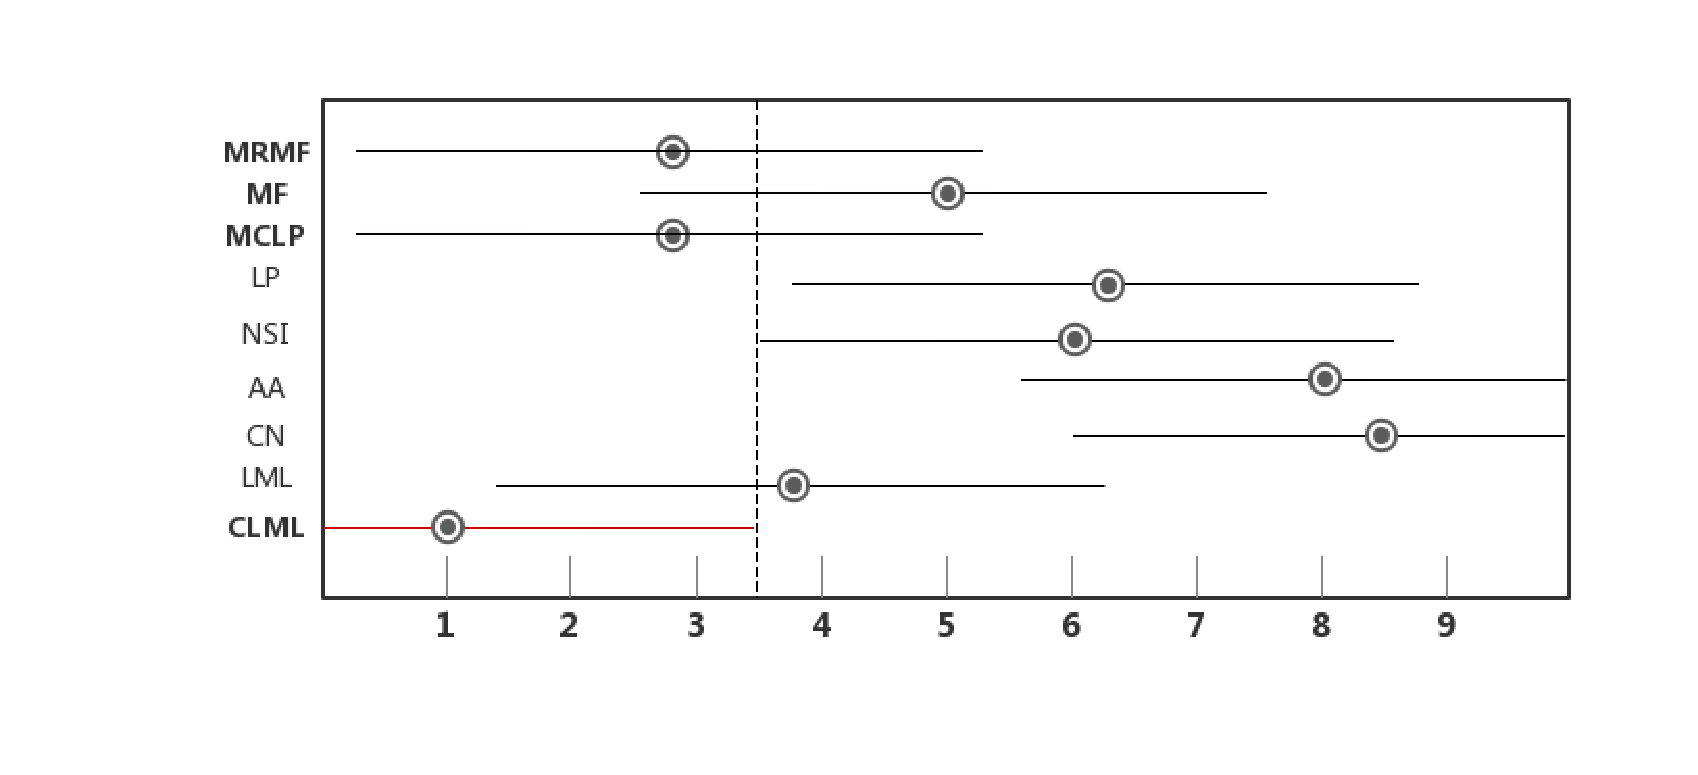
\includegraphics[width=0.9\linewidth]{post_hoc.pdf}
    \caption{弗里德曼检验图}
    \label{experiments:fig:post_hoc}
\end{figure}


在得到了算法在准确率相关的性能后,我们接着想到:算法的鲁棒性如何呢?
因为在概述中也提到过,要做链接预测的原因之一就是缺少足够的数据,如果我们的算法仅在数据丰富的情况下才能做出良好预测,那显然适用范围很窄。
在\ref{method:sec:collaborative}中我们指出,通过使用协同学习可以使数据不断富化从而很好地克服数据稀疏的问题,那么接下来我们将从实验的角度验证这一结论。


\subsection{算法鲁棒性实验}
为了验证算法鲁棒性,我们使用了\cite{cannistraci2013link}\cite{valverde2014link}\cite{hanley1982meaning}中的方法:
将所有矩阵(D、R、T矩阵)均随机删除同等程度的数据,再依次所有算法对其做预测得到删减数据后的结果,重复上述过程N次,每次删减不同程度的数据。
本次实验我们依次保留了80\%、60\%、40\%和20\%的数据,得到了如图\ref{experiments:fig:robust}的实验结果,其中横轴代表保留数据的比例,纵轴代表算法的AUC值。


\begin{figure}
    \centering
    \subfigure[DDI数据集]{
      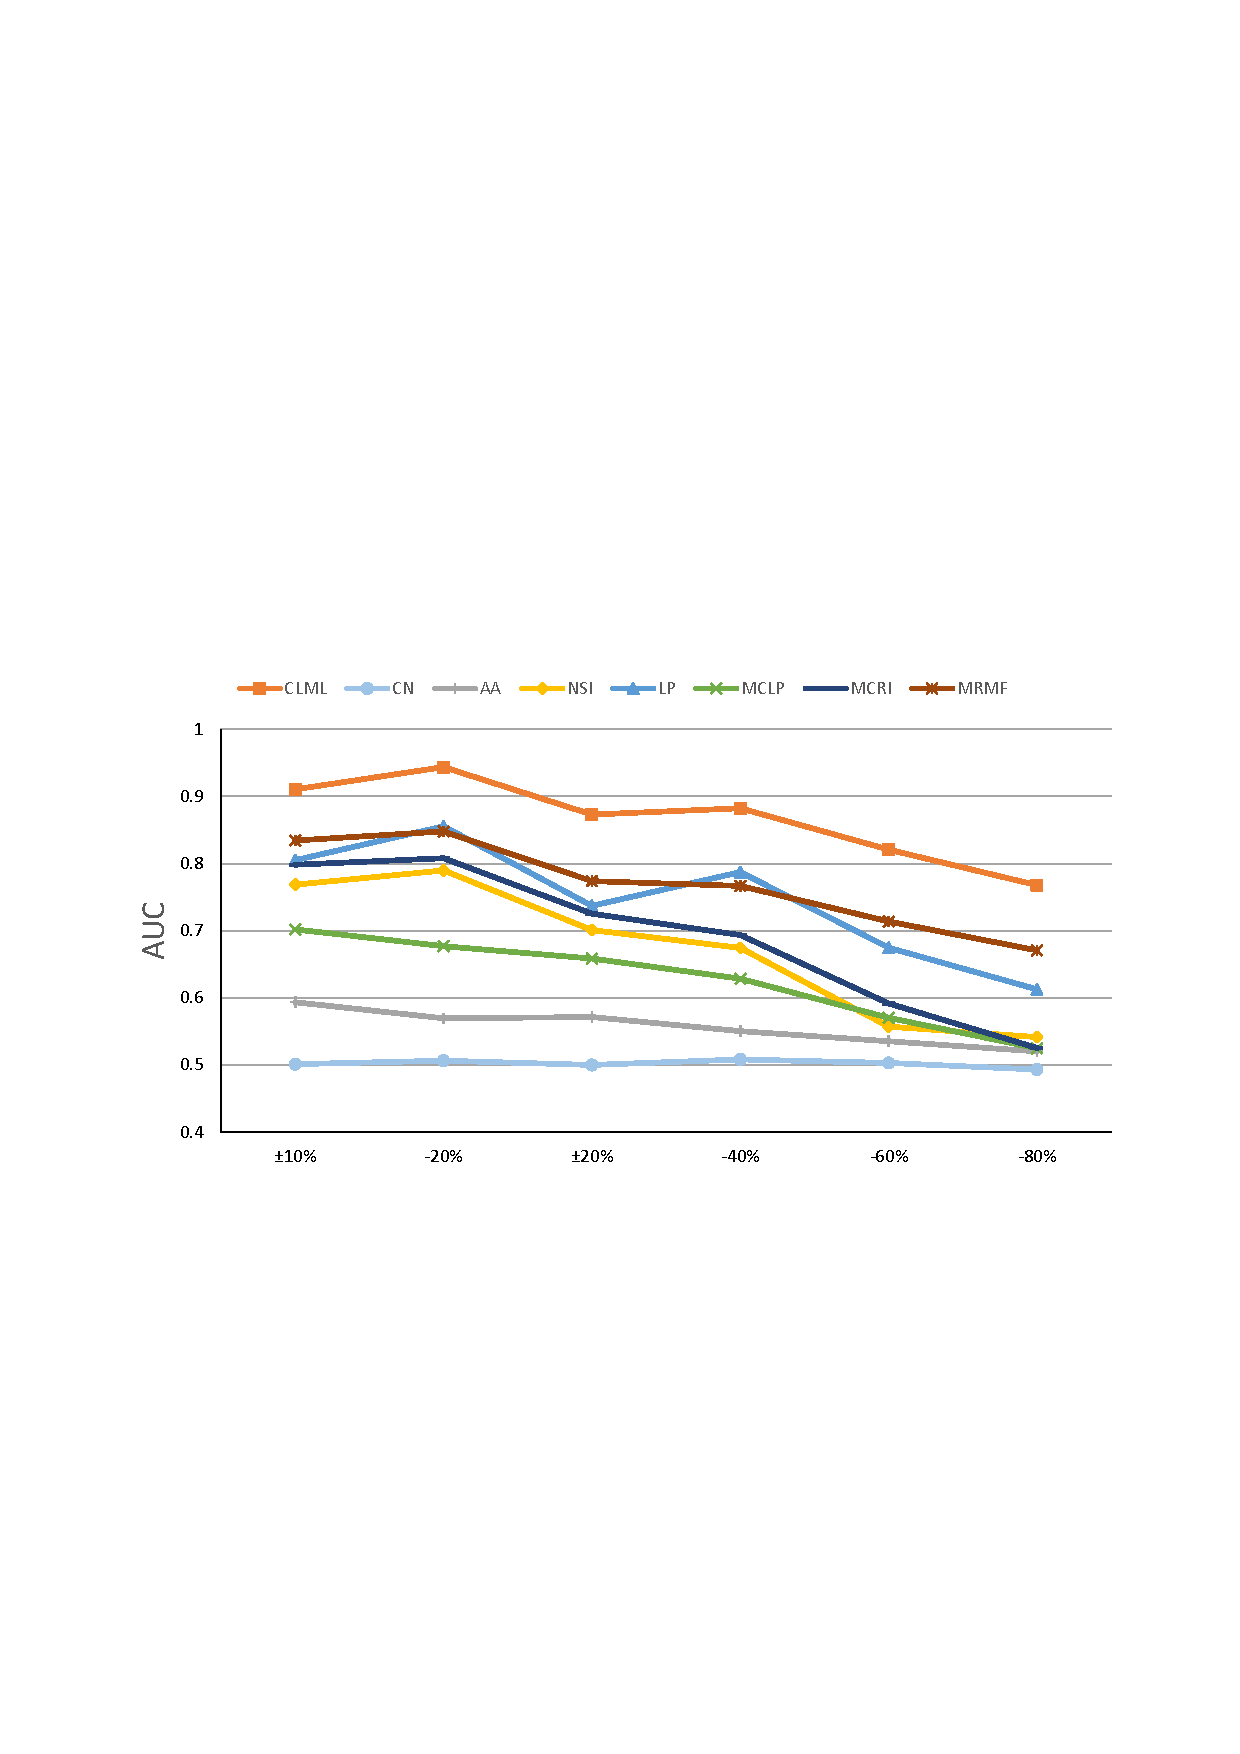
\includegraphics[width=0.45\linewidth]{AUC_DDI.pdf}
    }
    \subfigure[Yelp数据集]{
    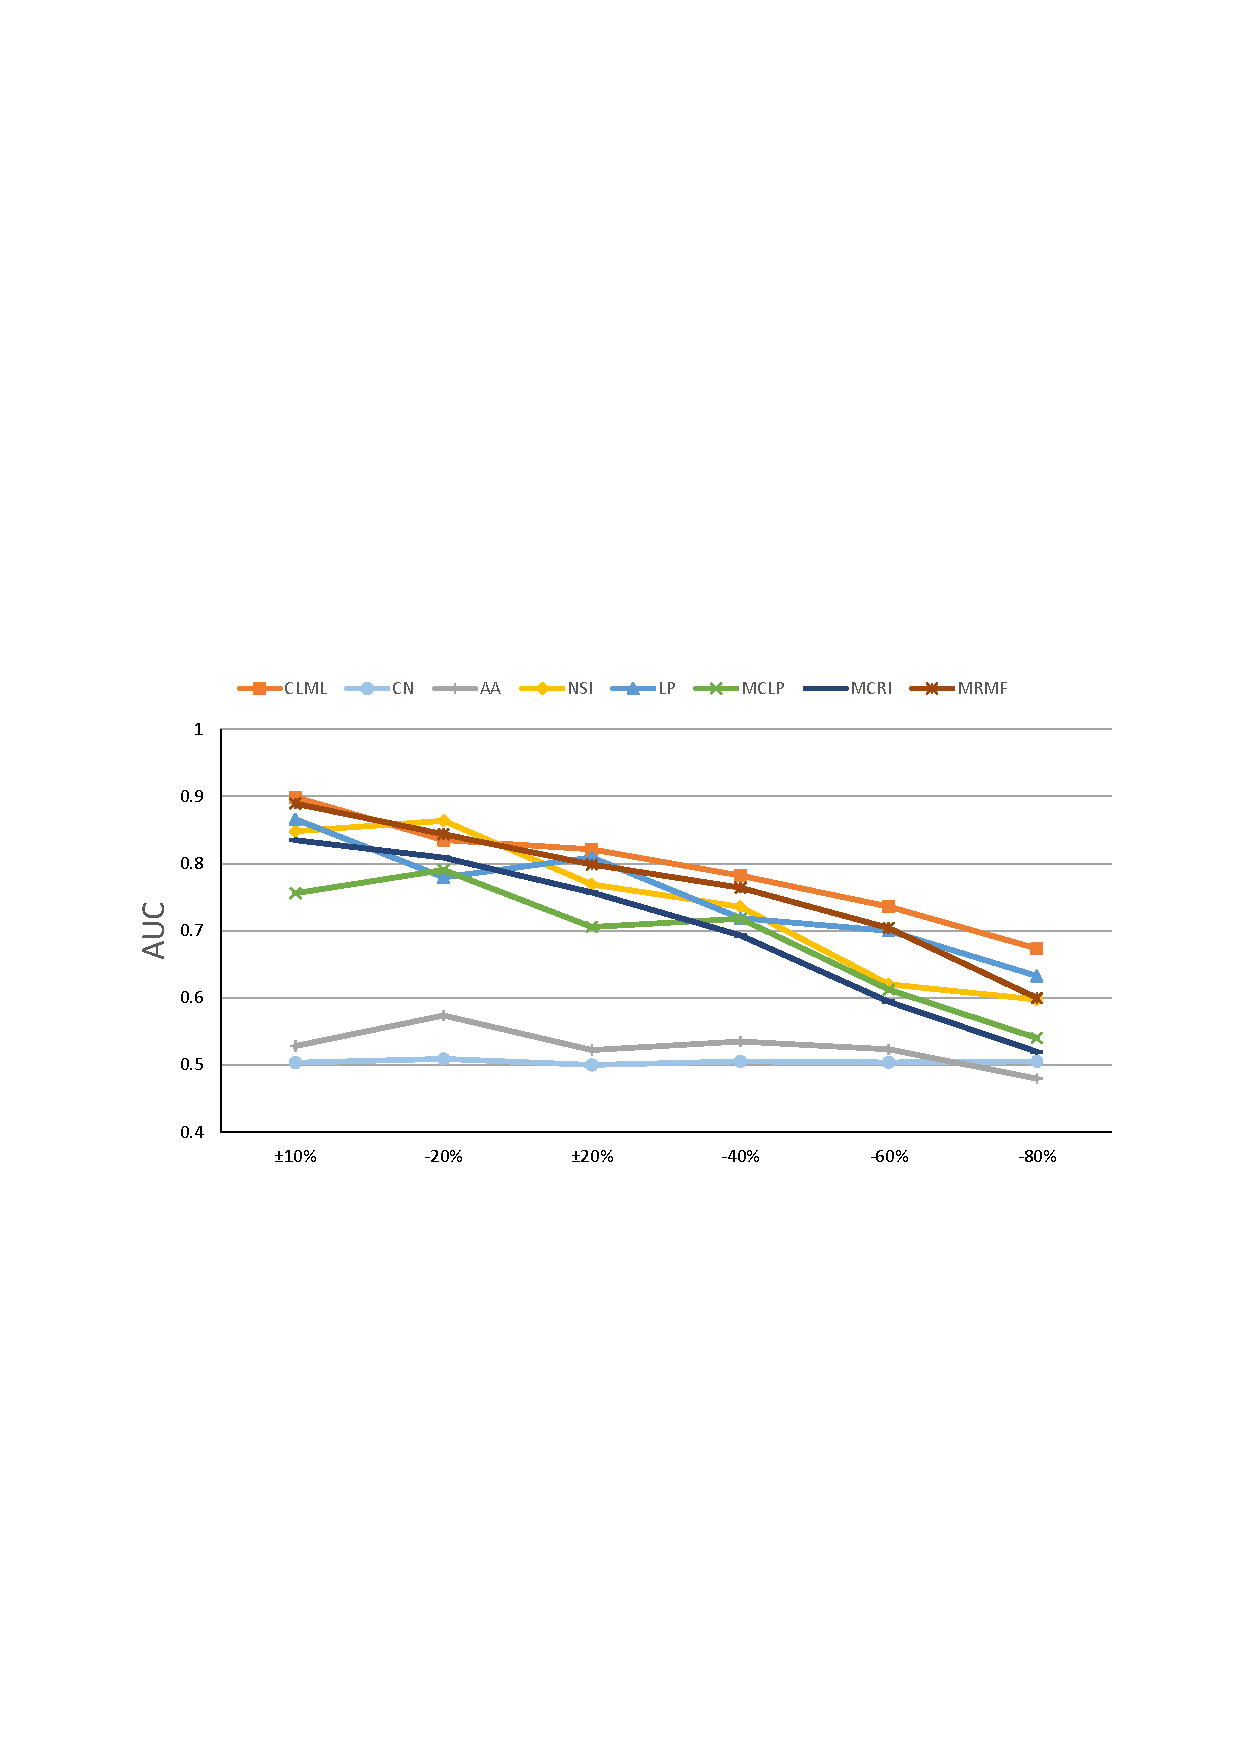
\includegraphics[width=0.45\linewidth]{AUC_Yelp.pdf}
    }
    \subfigure[Douban数据集]{
      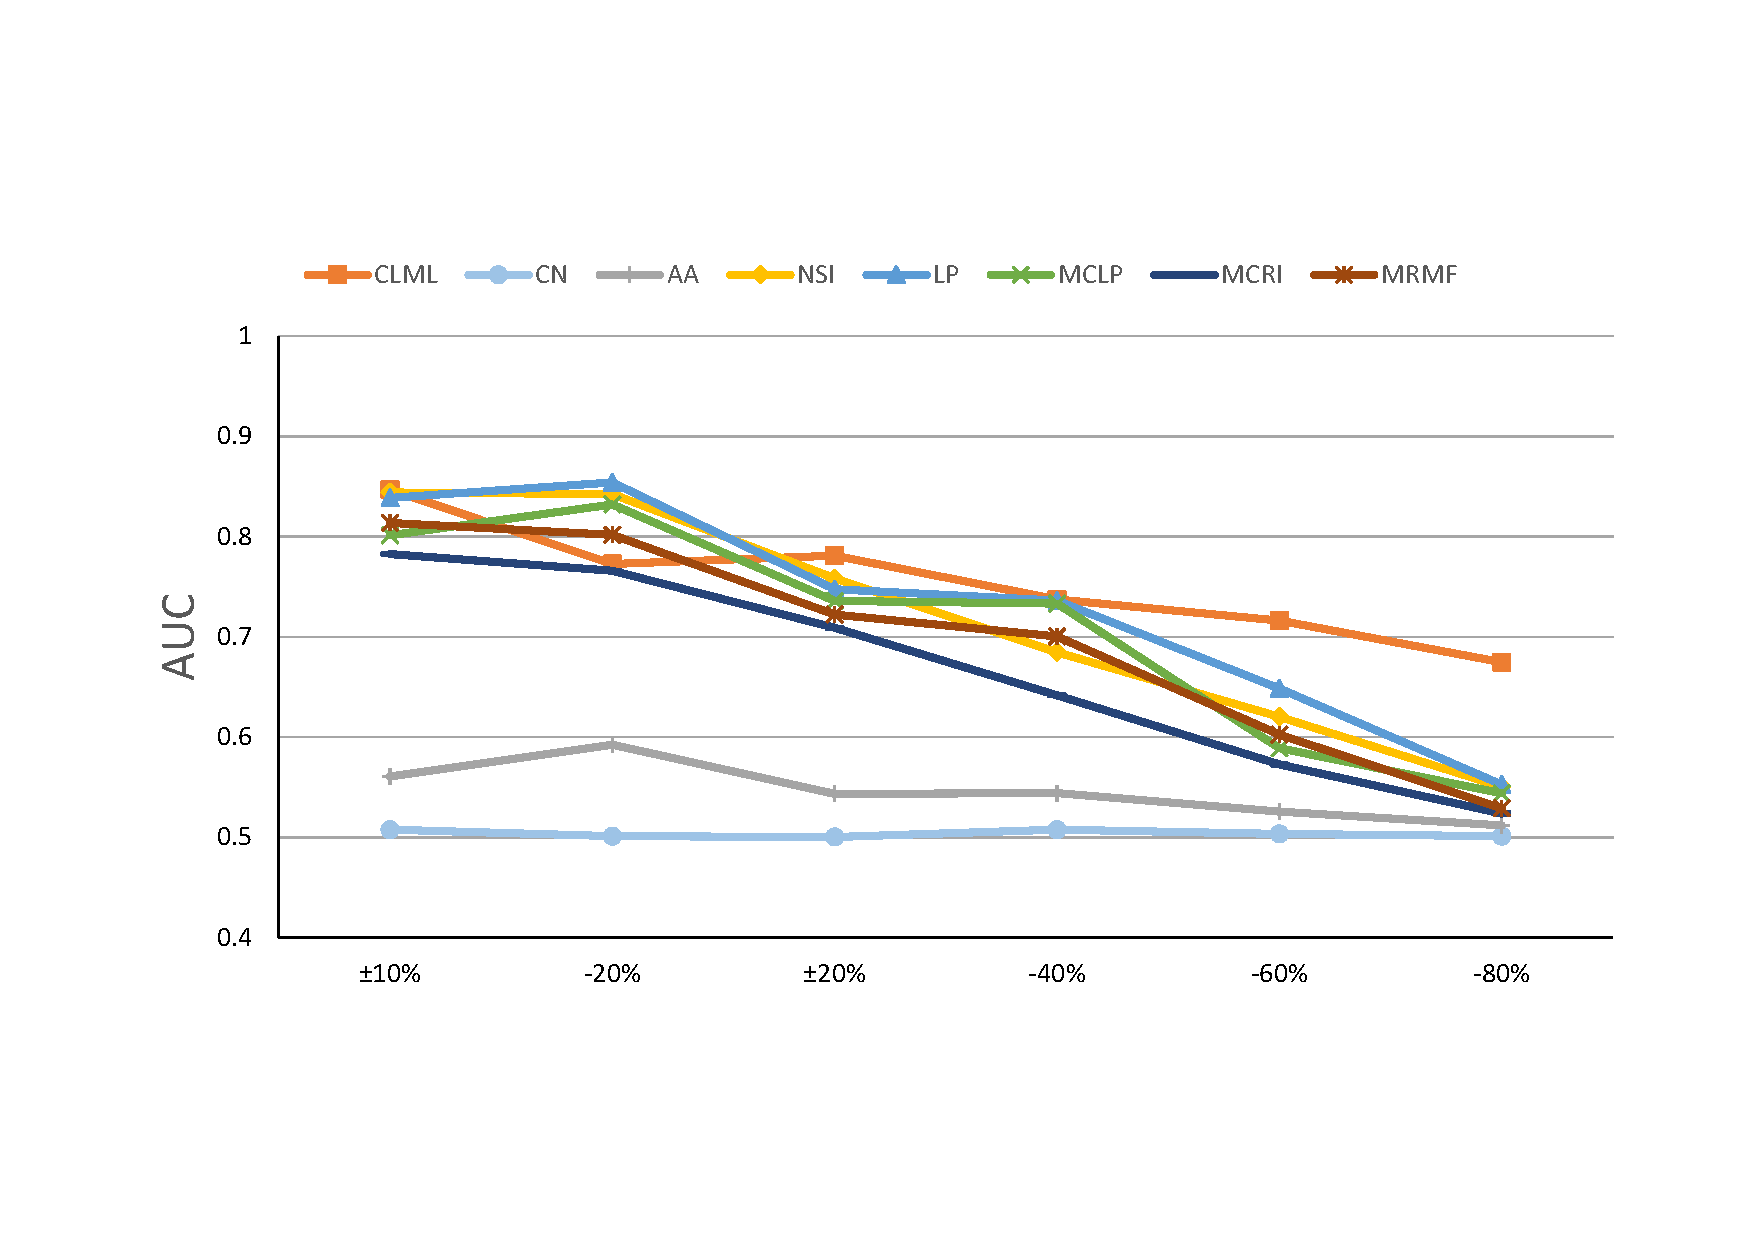
\includegraphics[width=0.45\linewidth]{AUC_Douban.pdf}
    }
    \subfigure[NIPS数据集]{
    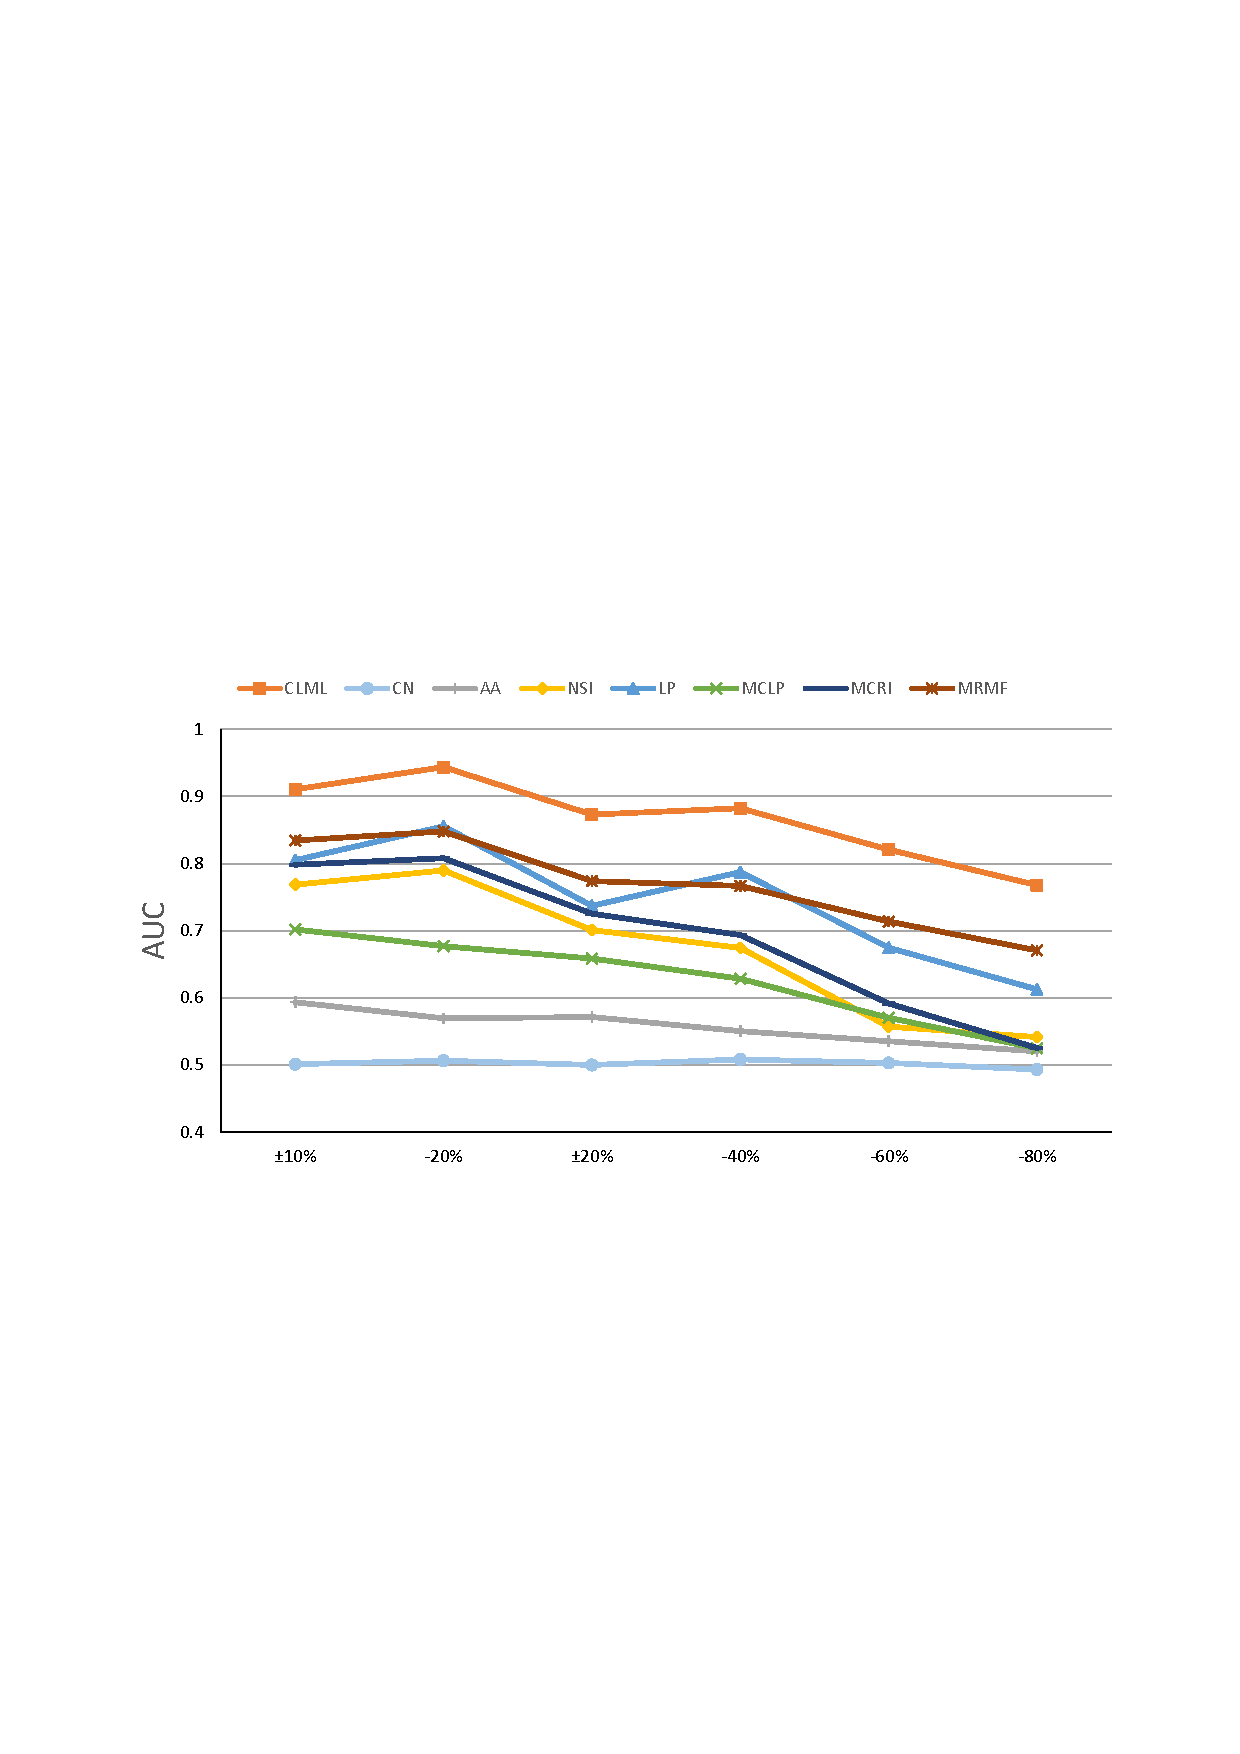
\includegraphics[width=0.45\linewidth]{AUC_NIPS.pdf}
    }
    \caption{算法在删减不同程度数据时的AUC}
    \label{experiments:fig:robust}
\end{figure}


从图\ref{experiments:fig:robust}中可以看出:
第一,所有算法的性能都会随着数据的缺失而有不同程度的下降,在数据仅剩20\%时AUC值最低;
第二,CLML的AUC曲线相对平缓,即下降速率相对缓慢,并且始终高于其它算法。
综上所述,我们可以说CLML算法的鲁棒性要优于其它算法。

\subsection{节点度数与算法性能的关系}
从图\ref{experiments:fig:robust}中我们还可看出,虽然CLML在各个数据集上的预测结果都优于其它算法,
但它本身在不同数据集上的预测结果仍有一定变化,因此我们希望知道数据结构特点和预测效果的关系。


在对式(\ref{method:formula:self_repre})的推导过程中提到,需要让空间中的每一个点(即D或T矩阵中的每一个元素)都将其用空间中的其余所有点线性表出,
且距该点距离越近的点权重越大,越远的点权重越小,而度数越高的点又拥有更多的近邻点。
由此产生一个问题,节点的度数会对预测准确率产生影响吗?是否度数越高的点,与其相关的预测准确率越高呢?


\ref{experiments:sec:db_cv}节中已经统计了数据集中具有不同度的节点数量,我们将对具有不同度的节点分别进行预测,
对于预测后数据中的每个点,设与点发生关联的概率最大的前五个点的集合为,
置与中每个点产生关联的概率为1,与其余点的概率置为0后便得到了一个0-1矩阵;这之后,将新构造出的矩阵与原矩阵对比,
若点与中的任一点在原矩阵中的关联概率仍为1则便认为对点预测成功,否则预测失败;
最后,设具有不同度的集合中的预测准确率为预测成功的点占集合的比例,作为最终结果。
实验的关键代码见代码3.2:



\begin{lstlisting}[caption={节点度数与算法性能的关系实验代码},language=Matlab]
    interaction = sum(D,2); %统计每个点的度

    [rows1,~] = find(interaction == 1);
    [rows2,~] = find(interaction == 2);
    ...
    [rows10up, ~] = find(interaction > 80);
    .... %其余实验设置
    % 开始预测
    predictData = abs(DualManifoldWithLowRank(R, trainData, 
    W1, T, W2, alphas(10), betas(1), gammas(10), maxIterator)); 
    predictData = predictData + predictData';

    [~, index] = sort(predictData, 1, 'descend');
    index = index(1:5,:); %选出前五个最可能发生关联的点
    count = 1;
    for i = 1 : samp_amount
    if(sum(D(index(:,i),i)) > 0) 
    % 若两集合有交集,则记录下当前的点
        results(count,1) = i;
        count = count+1;
    end
        
    end
    %统计成功预测出的不同度的点
    [result1,~,~] = intersect(results,rows1); 
    [result2,~,~] = intersect(results,rows2);
    ...
    [result10up,~,~] = intersect(results,rows10up);

    a1 = length(result1) / length(rows1); %预测准确率
    ...
    a7 = length(result10up) / length(rows10up);

\end{lstlisting}


因为节点数量会随着其度数增大而减少,为了实验稳定性,我们在度数大于5后对节点分段划分来做对比,
图\ref{experiments:fig:degree_auc}为初步实验的结果,其中横轴代表节点的度数,纵轴代表算法在每类节点上的预测准确率值。
从图\ref{experiments:fig:degree_auc}中可以看出,无论哪个数据集,预测准确率在具有更高度数的节点上的确会有所提升,这一点在DouBan数据集上尤为突出:
其准确率在度为1的节点中仅为0.5左右,几乎等于随机分类器的准确率;
但随着节点度数的上升,准确率有明显的提升直至最后稳定值0.88上下。


\begin{figure}
    \centering
    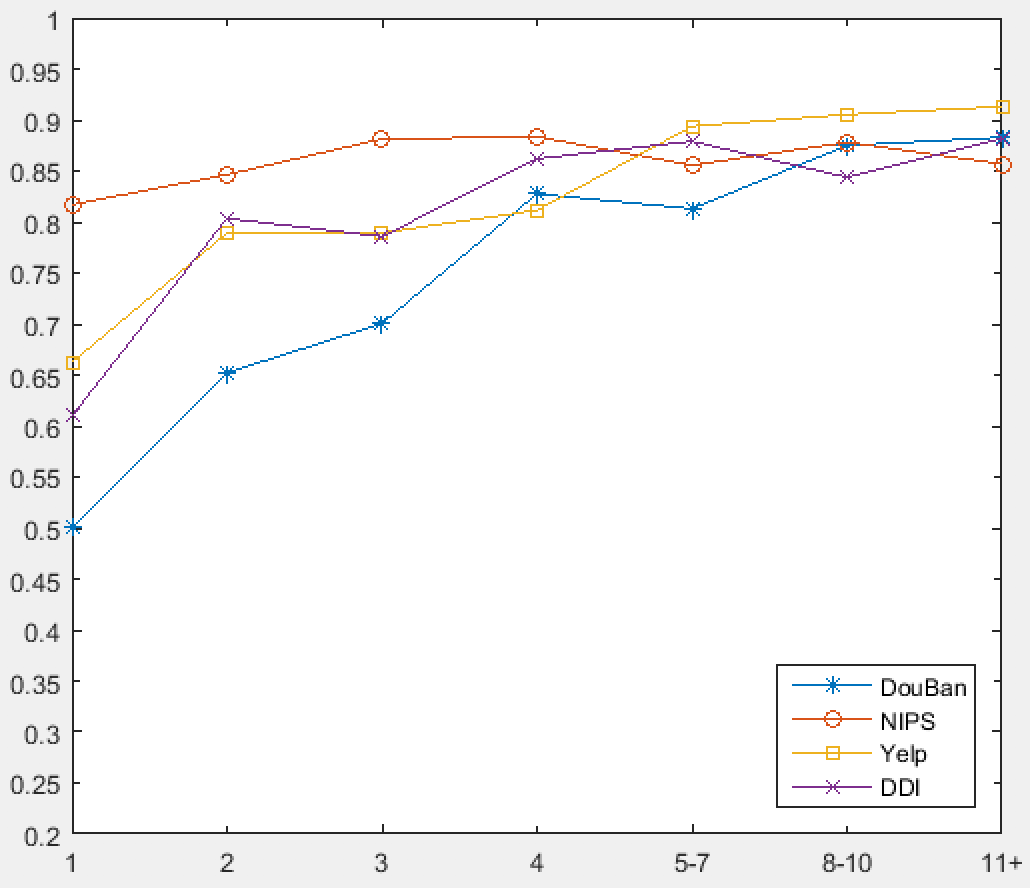
\includegraphics[width=0.6\linewidth]{degree_auc.png}
    \caption{节点度数和准确率的关系}
    \label{experiments:fig:degree_auc}
\end{figure}

但针对本次实验现象我们还存在一个疑问:
图\ref{experiments:fig:degree_auc}显示度数少的节点有非常多,而实验仅从中选取了少部分节点,而对于度数高的节点,因其数量很少故实验时使用了全部的数据,
那么曲线的上升是否是因为使用的训练数据比例提升了而不是因为节点的度数提升了呢?
为此我们针对Douban、Yelp这两个有较多低度数节点(因此训练数据比例也更低)的数据集做了进一步实验。


\begin{figure}
    \centering
    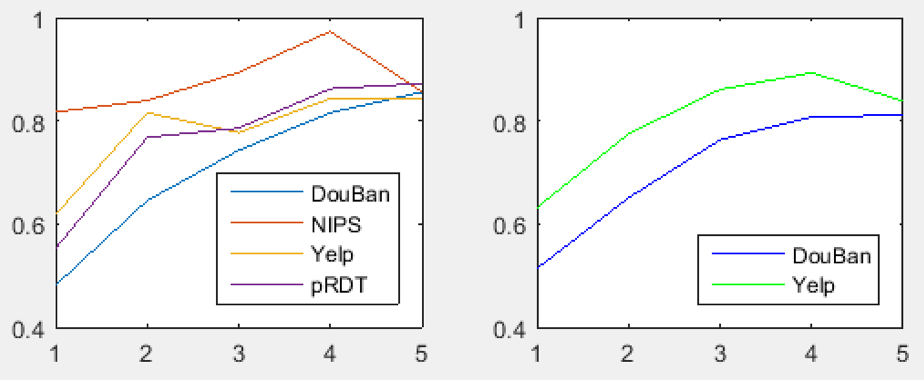
\includegraphics[width=0.85\linewidth]{degree_auc2.png}
    \caption{扩大对低度数节点的采样比例后的实验结果对比}
    \label{experiments:fig:degree_auc2}
\end{figure}

我们扩大了对低度数节点的抽取比例,若该做法可使算法对低度数节点的预测准确率有明显提升,
则我们可以认为图\ref{experiments:fig:degree_auc}中曲线的上升主要是由训练数据比例增大导致的,和节点度数无关。
提高了对度数为1、2、3的节点的抽取比例后得到的曲线(右)和原曲线(左)的对比如图\ref{experiments:fig:degree_auc2}。
从图中可看出,即使提高了部分节点的采样比例,曲线仍呈同样的上升趋势且在度数低的节点上的预测准确率并无显著变化,
因此我们可以对上述疑问作出否定回答,即预测准确率与采样比例并无明显关联。


\subsection{聚类系数与算法性能的关系}
在\cite{lu2011link}\cite{valverde2014link}中均提到,聚集程度较高的簇对算法结果有促进作用;
此外,聚集程度高的网络,其矩阵往往是低秩的,而CLML本身就假设了数据的低秩性并引入了低秩约束,而且这类网络本身就可能存在着更多的链接。
于是我们希望验证数据的聚集程度是否能对结果产生促进作用。
为此,我们在本次实验中使用了聚类系数\cite{barrat2000properties}来衡量矩阵的聚集程度,并观察算法对具有不同(全局)聚类系数的网络的预测结果是否会有差异。

实验时,我们每次随机从NIPS数据集中选取不同的数据形成固定大小的子集$D_i^{'}$,计算出该子集的聚类系数$CC_{D_i^{'}}$。
再依次使用不同的算法对该子集进行链接预测,得到每一个算法在$D_i^{'}$上的$AUC_{D_i^{'}}$。
重复上述步骤多次后,对于每一个算法我们都将得到一系列数据点,代表不同聚类系数下该算法的AUC值。
之后我们对这些数据进行线性拟合,便可得到一条有关聚类系数和算法性能关系的曲线。
图\ref{experiments:fig:cc_auc}展示了本次实验的结果,从图中可以看出:
首先,聚类系数高的数据集的确对算法结果有促进作用,这一点可通过在图中大部分算法的AUC都随着聚类系数的上升而上升;
其次,在所有算法中CLML在当聚类系数提高时,模型AUC值的提升效果更为显著,这一点可通过CLML曲线具有较高的斜率中看出。


\begin{figure}
    \centering
    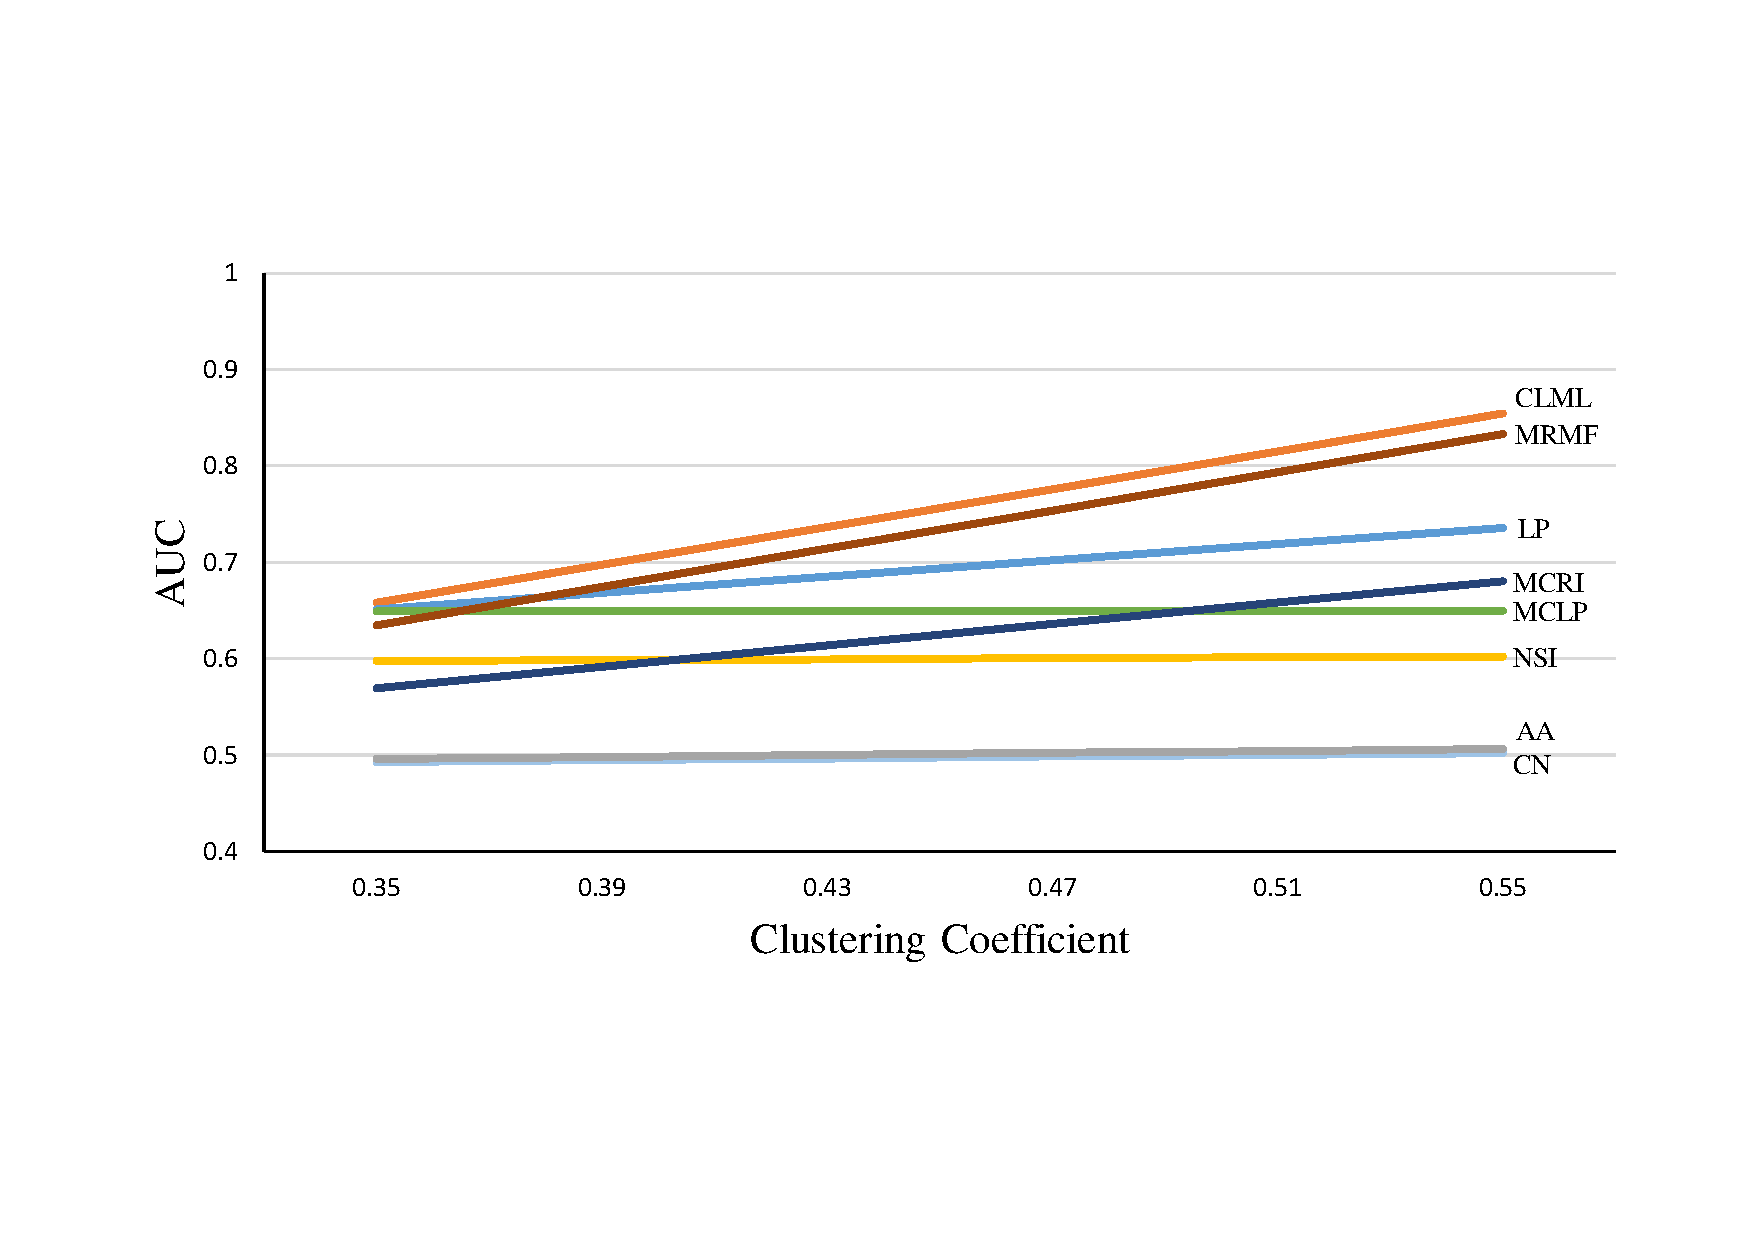
\includegraphics[width=0.99\linewidth]{CC_AUC.pdf}
    \caption{数据集聚类系数和算法AUC的关系}
    \label{experiments:fig:cc_auc}
\end{figure}


\subsection{案例分析}
在先前的实验中,我们在阐释CLML算法在各数据集上的结果时仅给出了如AUC、AUPR值这样抽象的数学结论。
而这一节为了进一步具体地看出CLML在实际应用中的价值,我们将CLML在做药物-药物关联预测时的结果从现实意义上做了分析,并将部分结果做了可视化处理。

在上文中提到,算法最终的结果是一个概率矩阵P,矩阵中的每个元素表示点i与点j产生关联的概率,在药物-药物关联预测中的意义即为药物i和药物j在临床使用时发生相互作用的概率。
为了验证CLML的实际意义,我们从预测结果中选取了前十个有着最大概率且未在Drugbank中收录的链接(相互作用),
并从Drugbank中找到了其对应的药物名称,如表\ref{experiments:table:case_study}所示。
在表中加粗的行表示其代表的相互作用已在其它论文、数据库或权威信息源得到了验证,
这些也可从Interaction Checker tool网站中检索到。
在这10个潜在关联中,有8个(80\%)已被验证为正确,这足以证明CLML算法在药物-药物关联预测这类实际应用场景下的有效性。
图\ref{experiments:fig:network}以表中所涉及的药物为例画出了与其相关的所有药物间的关系网络,节点颜色表示其度数,颜色越深则其度数越高;
方形节点为表\ref{experiments:table:case_study}中涉及到的药物,粗实线表示预测出且被验证为存在的关联,粗虚线表示预测出但尚未得到验证的关联

举例来说,在概述中提到,患有抑郁症等情绪障碍的患者需要长期服用抗抑郁类药物,而此类患者又往往伴随其它病灶,需要同时服用多种药物,因此导致抗抑郁类药物成为发生DDI的“主力军”。
在表\ref{experiments:table:case_study}的第七行中,我们预测出了一例由帕罗西丁(Paroxetine)与盐酸多奈哌齐(Donepezil)共同临床使用引起的相互作用,
其中前者就是一类被称为SSRIs的抗抑郁药物,在看到其临床效果之前可能需要数周的治疗,它和盐酸多奈哌齐会互相影响(抑制或促进都有可能)彼此的药物代谢作用从而影响到药效,
因此被建议临床使用时需有医生监控。

\zihaowu
\begin{center}
    \tablecaption{预测出的前十名最有可能发生的DDI}
    \begin{tabular}{ccc}\hline
    概率排名 & DrugBank ID & 药品名称\\ \hline
    \bfseries 1 & \bfseries DB00777, DB00674 & \bfseries Propiomazine, Galantamin \\
    \bfseries 2 & \bfseries DB01238, DB00674 & \bfseries Aripiprazole, Galantamine \\
    \bfseries 3 & \bfseries DB00777, DB00843 & \bfseries Propiomazine, Donepezil \\
    4 & DB00715, DB00382 & Paroxetine, Tacrine \\
    \bfseries 5 & \bfseries DB00777, DB00382 & \bfseries Propiomazine, Tacrine \\
    \bfseries 6 & \bfseries DB01238, DB00843 & \bfseries Aripiprazole, Donepezil \\
    \bfseries 7 & \bfseries DB00715, DB00843 & \bfseries Paroxetine, Donepezil \\
    \bfseries 8 & \bfseries DB01238, DB00726 & \bfseries Aripiprazole, Trimipramine \\
    9 & DB00382, DB01239 & Tacrine, Chlorprothixene \\
    \bfseries 10 & \bfseries DB00382, DB00420 & \bfseries Tacrine, Promazine \\ \hline
    \end{tabular}
    \label{experiments:table:case_study}
\end{center}
\zihaoxiaosi

\begin{figure}
    \centering
    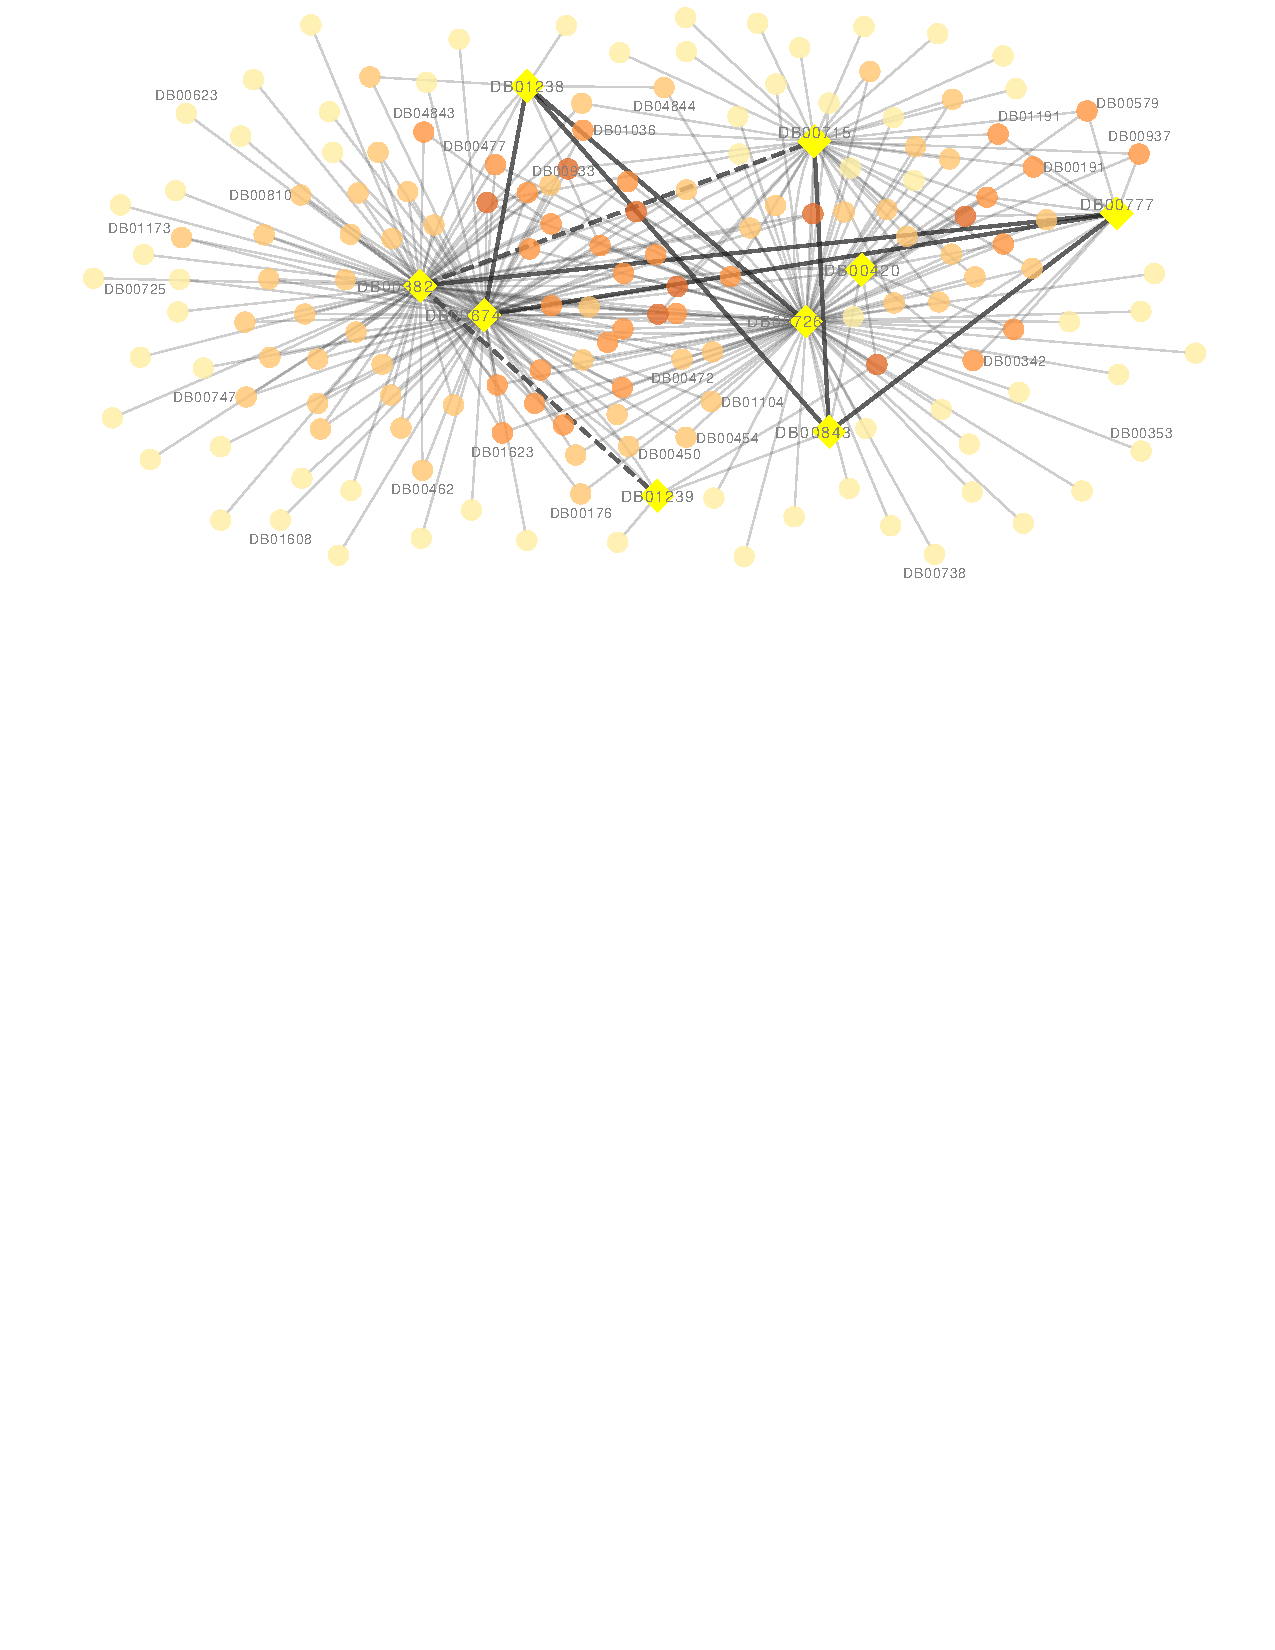
\includegraphics[width=0.95\linewidth]{network.pdf}
    \caption{药物互作网络的可视化图}
    \label{experiments:fig:network}    
\end{figure}


\section{本章小结}
在这一章中我们通过实验得到了CLML算法的各项性能,
其中通过实验一我们得到了CLML和其它比较算法在各个数据集上的AUC、AUPR等性能指标,并进一步用后续检验得出了CLML优于其它算法的结论;
通过实验二我们发现CLML较其它算法而言具有更好的鲁棒性;
实验三告诉我们,CLML在越密集的点(即度数越大的点)上预测准确率越高;
实验四在上一个实验的基础上又检验了数据集本身的聚集程度和准确率的关系,得出算法在聚集程度越高的数据集上预测效果越好的结论;
实验五将CLML实际应用到了药物-药物关联预测上,从现实意义上分析了实验结果并将结果做了可视化。
综合以上各个实验的结论后我们可以看出,CLML算法从整体性能上就要优于其它对比算法,且在实际问题中依然很有效率。

% !TeX root = ../main.tex
% -*- coding: utf-8 -*-
\chapter{总结与展望}
实现本篇论文的工作主要分为三部分:首先是调研了相关文献来了解链接预测的背景、经典算法以及近些年提出的较有代表性的算法,并在之后提出了自己的算法;
之后设计了一系列实验来验证算法的性能,并根据实验现象对算法做了调整,最终得到了完整的算法模型及其在实际问题中的应用效果;
最后用一些实验从数据的角度上探究了影响算法性能的几个因素。


未来的工作也许可以从以下几点入手:
第一,在研究网络聚集程度对算法性能的影响中,实验并不充分,得出“网络聚集程度越高,算法准确率越高”的结论还需要扩大对数据集聚类系数的选取范围,并增大数据量;
第二,实验中未考虑数据集间噪声的不平衡性,日后可以从添加噪声和降噪这两个角度来平衡数据集间的噪声差异;
第三,在所有评估算法性能的实验中,均为提及运行时间这一指标。事实上,受算法复杂性影响,CLML需要很长的运行时间,
这一点和其它算法对比时是一个劣势,今后也许可以对运行效率做进一步优化。
% !TeX root = ../main.tex
% -*- coding: utf-8 -*-

\printbibliography

% !TeX root = ../main.tex
% -*- coding: utf-8 -*-

%\makeschapterhead{致谢}
\chapter*{致谢}
在本篇论文的最后,我要对所有帮助我完成论文的老师及同学真诚地表示感谢。


首先,我要对我的导师谢茂强老师由衷地表示感激之情。
在指导我做毕业论文之前,谢老师在课上对大学教育的看法、对我们的寄托甚至老师的自我反省就已经对我产生了深刻影响,让我对老师产生了深深的敬意。
在指导我做毕业论文的时候,即使是小问题老师也会专门留出时间耐心地为我解答,对于论文的看法老师会认真倾听我的想法后再与我交流沟通,最终一步步推进着工作顺利完成。


同时,我也要感谢刘嘉晖和刘帆师兄。是两位师兄带领我走进科研世界,耐心细致地解答我的疑惑,并指导我做完了所有实验。
我从他们身上学到了很多东西,在实验室度过了非常快乐的时光,他们不仅是我的师兄更是我的好朋友。


最后,感谢本科这四年中帮助过我的所有同学、室友和赵欣璇,是你们陪伴我度过了如此美好又难忘的大学时光,
也是你们教会了我如何思考、如何与人相处、如何规划人生,让我慢慢成长到今天。


\end{document}
